% Modified for use with JCC - Madhusudan Singh Copyright (C) (2012). All rights reserved.
%\documentclass[aip,reprint]{revtex4-1}
\documentclass[aip]{revtex4-1}

\setlength{\oddsidemargin}{0in}  %left margin position, reference is one inch
\setlength{\textwidth}{6.5in}    %width of text=8.5-1in-1in for margin
\setlength{\topmargin}{-0.5in}    %reference is at 1.5in, -.5in gives a start of about 1in from top
\setlength{\textheight}{9in}     %length of text=11in-1in-1in (top and bot. marg.) 
%\newenvironment{wileykeywords}{\textsf{Keywords:}\hspace{\stretch{1}}}{\hspace{\stretch{1}}\rule{1ex}{1ex}}

\usepackage{amsmath,amssymb}
\usepackage{graphicx}% Include figure files
%\usepackage{caption}
\usepackage{color}% Include colors for document elements
\usepackage{dcolumn}% Align table columns on decimal point
\usepackage{bm}% bold math
%\usepackage[numbers,super,comma,sort&compress]{natbib}
%\usepackage[nolists, nomarkers, figuresfirst]{endfloat}

\definecolor{background-color}{gray}{0.98}
\graphicspath{{data/}{images/}}

\begin{document}

%\title{Atomic pseudo-potentials for sp$^2$ carbon atoms}
\title{Atomic pseudo-potentials for reproducing the valence electron behaviour of sp$^2$ carbon atoms}
\author{Alexander Punter}
\author{Paola Nava}
\author{Yannick Carissan}
\affiliation{Aix Marseille Univ, CNRS, Centrale Marseille, iSm2, Marseille, France}

\begin{abstract}
A pseudo-potential system for recreating an sp\(^{2}\) carbon atom is built 
and tested as a building block for various pseudo-hydrocarbon chain and ring systems.  
This pseudo-system has a central charge of one, thus it contains only one
electron. It is employed in \textsl{ab-initio} calculations on a variety of hydrocarbons, from small chains to polycyclic aromatics.
The relative errors obtained with the PBE0 functional range from
1.0\% on TD-DFT first excitation energy to 10\% on ionisation
energy.
\end{abstract}
\maketitle
%\begin{wileykeywords}
%Anisotropy, Pseudo-potential, $\pi$ system, Quantum Chemistry, Spin %contamination
%\end{wileykeywords}

%*****************Graphical Table of Contents******************** THIS IS MANDATORY *******************


\begin{figure}[h]
\centering
\colorbox{background-color}{
\fbox{
\begin{minipage}{1.0\textwidth}
%\includegraphics[width=50mm,height=50mm]{cc.eps} % Pick only one of the two styles by uncommenting the corresponding \includegraphics
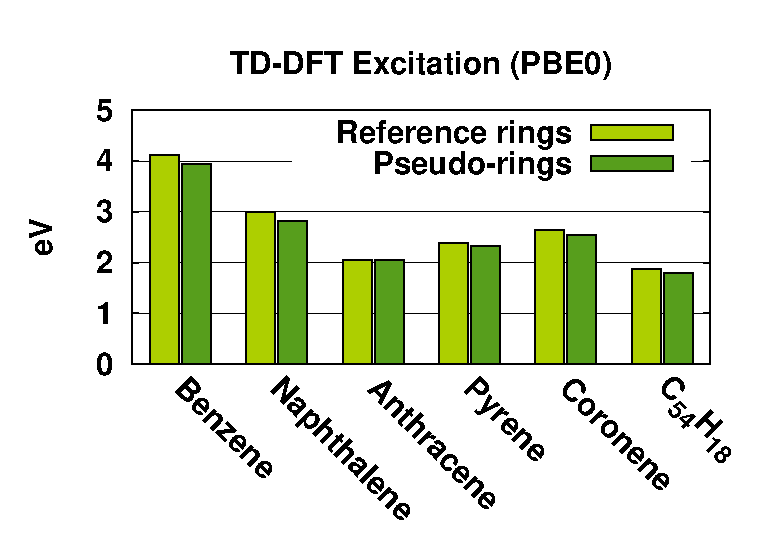
\includegraphics[width=50mm]{ring_pbe0_tddft}
%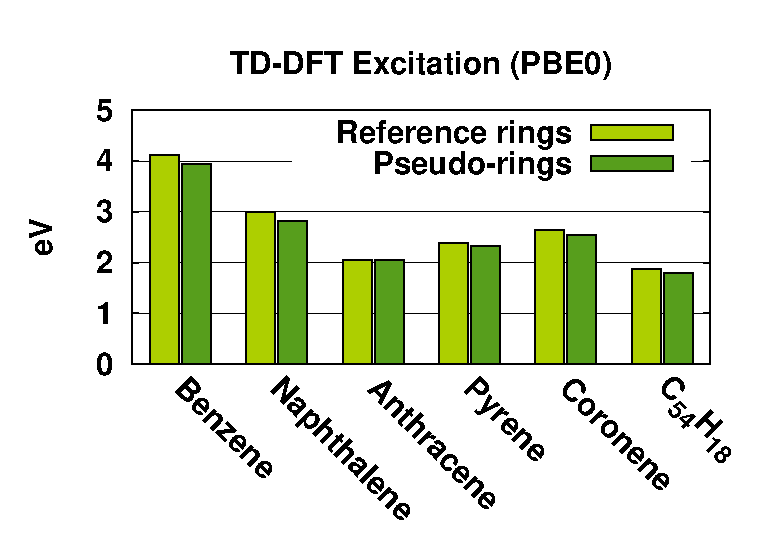
\includegraphics[width=110mm,height=20mm]{ring_pbe0_tddft}
\\
A pseudo-potential system for recreating an sp\(^{2}\) carbon atom is built 
and tested as a building block for various pseudo-hydrocarbon chain and ring systems.  
This pseudo-system has a central charge of 1, thus it contains only one
electron. It is employed in \textsl{ab-initio} calculations on a variety of hydrocarbons, from small chains to polycyclic aromatics.
The relative errors obtained with the PBE0 functional range from
1.0\% on TD-DFT first excitation energy to 10\% on ionisation
energy.
\end{minipage}
}}
\end{figure}

% makes references listed with 1., 2., etc.  
  \makeatletter
  \renewcommand\@biblabel[1]{#1.}
  \makeatother

\bibliographystyle{apsrev}

\renewcommand{\baselinestretch}{1.5}
\normalsize


\clearpage
% 

\section{Introduction}
\newcounter{customItem}
\newcommand{\showCustomItem}{\refstepcounter{customItem}\roman{customItem}}

%For most of the quantum chemistry calculations, the system can be divided into two parts:
%the active part, \emph{i.e.} the part of the molecule one is interested in and
%the inactive part, which is to be taken into account in order to fulfill chemical requirements.
It is a common idea that a chemical system can be thought of as comprised of
two parts:
an active one, where most of the chemistry takes place, and an inactive
one, which must be taken into account in order to fulfill chemical requirements.
Based on this general statement, many successful theoretical approaches have been developed.
Among them can be cited QM/QM' or QM/MM methods (\showCustomItem), where 
the active region that usually contains several atoms is
treated at a high level of calculation, while the inactive part is treated at a 
lower level of theory.\cite{chung_oniom_2015}
Fragmentation methods split the complete problem into smaller parts and combine individual calculations
on these fragments to recover the properties of the overall system.\cite{gordon_effective_2001,steinmann_effective_2012}
Frozen density embedding techniques (\showCustomItem) replace part of a molecule, or 
its surroundings,
by a frozen electronic density extracted on a reference system.\cite{wesolowski_frozen-density_2015}
They are an extension of the frozen core approximation, already used to reduce
the number of parameters to be optimised in the self consistent field calculation.
In the framework of this work, the pioneering work of Rivail \emph{et al.} must be mentioned:
the total wave function is optimised with some molecular orbitals kept frozen.\cite{ASSFELD1996100}

In this article we shall focus on pseudo-potential techniques, which also
divide the chemical problem into two parts.
Effective core potentials (\showCustomItem) are commonly employed for atoms: 
core electrons (and effects due to the corresponding nuclear charge) are
replaced by an operator which is quick to evaluate, and the active electrons are treated
explicitly.\cite{dolg_relativistic_2012}
In the same vein, model potentials (\showCustomItem) replace a frozen electronic density (computed from the atom)
by a series of operators, which depend on the level of
refinement required.\cite{huzinaga_1994_1995}

The effective group potentials (\showCustomItem) bridge the frozen density and the core potential
approaches: using core potential extraction techniques, effects due to the implicit 
electron density (and corresponding nuclear charge) 
are reproduced by a mono-electronic operator.\cite{carissan_what_2006, raynaud_multicentered_2010}
However, while effective core potentials and model potentials intend to 
reproduce atomic properties,
effective group potentials aim at mimicking the effect of atoms involved in one or more chemical
bonds. The cyclopentadienyl group has, for instance, been successfully extracted.\cite{carissan_what_2006}
In this example, the active part consisted of six electrons (the $\pi$ electrons) and six
nuclear charges, with the pseudo-potential replacing all the rest, including the hydrogen atoms.
Even if the $\sigma / \pi$ separability suggested how to define the active and the inactive parts,
carbon atoms are hybridised and the core/valence distinction is not 
strictly defined.

The theoretical background to extract effective group pseudo-potentials  can be traced back 
to several contributions in the 80's and  90's.\cite{Nicolas1980a, huzinaga_effective_1991, huzinaga_1994_1995, EGP5, EGP6, EGP9}
In 1992 Katsuki built molecular potentials based on Huzinaga's model potentials.\cite{katsuki_molecular_1992,katsuki_spectral_1993}
 In his work on this subject, Huzinaga emphasises that pseudo-potentials should maintain three effects of the
'dormant' electrons on the active ones: the Coulomb, the exchange and the 'no-collapse' term.\cite{huzinaga_effective_1991}
Following his proposal, for an atom where active and dormant electrons have been separated, the Hamiltonian reads:
\begin{equation}
\label{eq:atomicHamiltonian}
\hat{H} = \sum_{i=1}^n \hat{h}(i) +\sum_{i<j}\frac{1}{r_{ij}}
\end{equation}
with $\frac{1}{r_{ij}}$ the bi-electronic interaction
between explicitly treated active electrons and
the mono-electronic operator:
\begin{equation}
\label{eq:monoElectronicOperator}
%\hat{h}(i) = -\frac{1}{2}\Delta_i - \frac{(Z-Z_c)}{r_i}+\hat{V}(i) + \hat{\sigma}(i)
\hat{h}(i) = -\frac{1}{2}\Delta_i - \frac{(Z-Z_c)}{r_i} + \hat{W}
\end{equation}
where $\Delta_i$ is the Laplacian of the coordinates of electron $i$, and 
$Z_C$ is the number of core electrons withdrawn from the reference system.
The operator $\hat{W}$ contains two terms: the 
$\hat{\sigma}$  'no-collapse' term that prevents active electrons
collapsing into the dormant region and the operator $\hat{V}$ that reproduces the 
Coulomb and exchange interactions:
\begin{equation}
\label{eq:HuzinagaMPVersion1Potential}
\hat{V} = \frac{1}{r}\left[\sum_IA_I\exp(-\alpha_I r^2)+\sum_JB_Jr\exp(-\beta_J r^2)\right]
\end{equation}

To take into account the fact that dormant electrons are removed from the
system, the nuclear charge is modified by the $Z_c$ value.
Yet, as the effective charge felt by the active electrons is likely not to be an integer,
the modification of the value of the nuclear charge is scaled in $\hat{V}$.
In this operator we notice that the \(r^{-1}\) behavior is maintained for the first term 
(the Coulomb one).

In the present work, the aim is 
to propose a methodology for extracting a potential for
a hybridised carbon atom (here an $sp^2$ carbon atom), which can then be
used as a building block for constructing chemical systems. This carbon atom
will contain exactly one explicit nuclear charge and one explicit electron.
Moreover, the method should be usable 
out of the box in any standard quantum chemistry software.
Thus, no modification of the source code should be done.
This supplementary constraint will be fulfilled by strategically positioning in space the pseudo-potentials
we intend to use. 
The replacement of bi-electronic interactions with a set of mono-electronic integrals
will result in drastic gains in timings, a study of which is available in the supplementary material.
However, the main purpose of the current work is not to study the time gain from the use of our pseudo-potentials but to show that our approach of extracting pseudo-potentials
for hybridised atoms is possible with strictly local pseudo-potentials.

Pseudo-potentials for hybridised carbon
atoms have been already successfully extracted in a previous work of ours.\cite{drujon_pseudopotentials_2013}
There, our attention was focused on the 'no-collapse' term, and 
functions in the pseudo-potential shift up unwanted orbitals and correctly place the energy of the
wanted orbitals.
A drawback of this method was that some pseudo-potentials had to be put precisely at the center
of each bond.
Thus, those pseudo-potentials could not be considered as purely local as they were not defined solely
with respect to the position of the atom they applied to.
This previous work should therefore be regarded as a proof-of-concept.
In this new version, we include more physical meaning in our model, 
by placing pseudo-potentials that mimic Coulomb interactions among both the active and dormant electrons, and the shielded nuclear charge. 
The new pseudo-potentials are fully atomic: when replacing a hybridised atom, the atom's position and orientation can determine completely the placement of the potentials (as hybridisation destroys isotropy, the preferred orientations
must be given to define the pseudo-potential).

This article is structured as follows.
The first part (Methodology) gives the general definition of the pseudo-potential, which we subsequently develop.
Secondly, the particular case of the CH$_3^\bullet$ radical is detailed as it gives access
to some physically grounded values.
In a third part, the optimal pseudo-potential is defined. Details of the step-by-step extraction
are given in the supplementary material.
The application part focuses on the performances of the optimal pseudo-potential.
It is shown that the properties can be well reproduced except when dealing with
systems in which spin contamination is large.
For these cases, a solution is provided.

\section{Methodology}

\subsection{General pseudo-potential definition}

We make use of two kinds of gaussian pseudo-potentials \cite{me_structure_theory}, of \(s\) and \(p\) shapes. As we want to avoid modifying the quantum chemistry software itself, the pseudo-potentials have a semi-local form.
For a pseudo-carbon atom,
the multi-centered pseudo-potential that we built reads as follows:
\begin{align}
\label{eq:ourPP_init}
\hat{W} =&
\underbrace{\frac{1}{r} A\exp(-\alpha r^2)\sum_{m=-1}^{m=+1}\left|Y_{1,m}\right>\left<Y_{1,m}\right|}_{p \ \text{projector}}%
+\\
&\underbrace{\sum_J \frac{1}{r'_J} A'_J\exp(-\alpha'_J (r'_J)^2)\left|Y_{0,0}^J\right>\left<Y_{0,0}^J\right|}_{s \ \text{projectors}}%
\nonumber
\end{align}
The $p$ projector is centered on the pseudo-atom and it is entirely defined by the $A$ coefficient
and the $\alpha$ exponent, $Y_{1,m}$ are the $p$ real solid harmonics. The $s$ projectors are
placed around the pseudo-atom. The $J^{th} \ s$ projector is defined by its $A'_J$ coefficient, its
$\alpha'_J$ exponent and its position relative to the pseudo-atom, so that $r'_J = r-r^0_J$ with
$r^0_J$ the distance to the pseudo-atom. $Y_{0,0}^J$ is the $s$ real solid harmonic placed on
the $J^{th}$ center.
%$\alpha'_J$ exponent and its position $r^0_J$ relative to the pseudo-atom, so that $r'_J = r-r^0_J$.
%$Y_{0,0}^J$ is the $s$ real solid harmonics centered at $r^0_J$.

By analogy with Huzinaga model potentials defined in (\ref{eq:HuzinagaMPVersion1Potential})
we can say that our projectors have a coulombic nature.
%are built to mimic coulombic interactions.
%As will be discussed in the following sections,
The \(p\) pseudo-potential allows us to reproduce atomic properties (see hereafter), while the
\(s\) potentials mimic electrostatic electron pair repulsion, in particular they 
recover part of the bi-electronic interaction
between the dormant and the active electrons. The pseudo-potentials are mono-electronic operators, thus they shall not be able fully to reproduce bi-electronic interactions. Knowing this, we adjust the parameters of the \(s\) potentials for the pseudo-system to have a wavefunction in which relevant properties, such as spatial extent, energy and excitation energies, are as close as possible to those of the reference system.

\subsection{Extraction for the CH$_3^\bullet$ radical}
\label{section:potential_derivation}

In a first step we use the planar CH\(^{\bullet}_{3}\) (d$_{CH}=2.0466$ $a.u.$, HF/def-SV(P)) as 
a case study.
It is the smallest system containing one and only one sp$^2$ hybridised carbon atom.
This will provide us with physically meaningful parameters, which are then employed as
initial guess for the extraction of a pseudo-potential for a general $\pi$ carbon atom.

\begin{figure}
\begin{center}
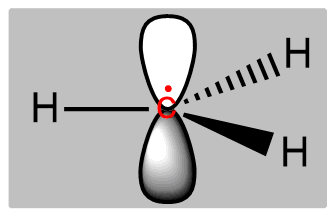
\includegraphics[width=8cm]{ch3.png}
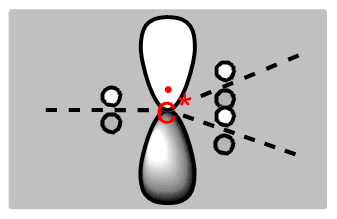
\includegraphics[width=8cm]{pseudoch3.png}
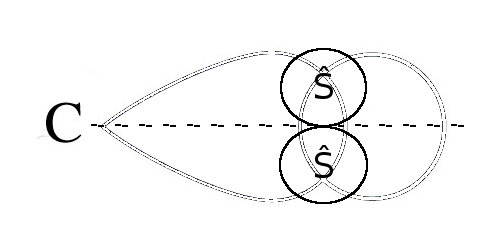
\includegraphics[width=8cm]{tm_sp2_potentials.png}
\end{center}
\caption{Diagrams of CH\(^{\bullet}_{3}\) (left) and pseudo-CH\(^{\bullet}_{3}\)
(right, below) molecules.
The pseudo-CH\(^{\bullet}_{3}\) diagrams display the \(s\) and \(p\) potential positions,
and the distances \(d\) and \(c\). White potentials are above the $xy$ plane, 
gray potentials are below.
In this article $d=0.5\;a.u.$ and $c=0.25\;a.u.$}
\label{figure:ref_pseudo_diagram}
\end{figure}

Figure \ref{figure:ref_pseudo_diagram} displays the final pseudo-system: the CH\(^{\bullet}_{3}\) radical has been replaced by
a hydrogen-like "pseudo-carbon", with a nuclear charge of \(Z_{nucleus} = 1\), and one electron occupying the \(p_{z}\) orbital. 
There are now no H atoms, and the system is surrounded by three potential pairs at a planar distance of \(d\), each consisting of 
two \(s\)-shaped potentials with a distance of \(c\) above and below the \((xy)\) plane. 
A further \(p\)-shaped potential is applied directly to the pseudo-carbon.
Based on Equation~\ref{eq:ourPP_init}, the complete pseudo-potential reads as:

\begin{align}
\label{eq:ourPP}
\hat{W} =&
\frac{1}{r} A\exp(-\alpha r^2)\sum_{m=-1}^{m=+1}\left|Y_{1,m}\right>\left<Y_{1,m}\right|%
+\\
&\sum_{J=1}^{6} \frac{1}{r'_J} A'\exp(-\alpha' (r'_J)^2)\left|Y_{0,0}^J\right>\left<Y_{0,0}^J\right|%
\nonumber
\end{align}

In this article, we fix \(c = 0.25\;a.u.; d=0.5\;a.u.\), Table~\ref{tab:pos}.
This gives us four variables to manipulate the properties of the system, 
notably the $A$ coefficient and the $\alpha$ exponent for the $p$ potential, and
the $A'$ coefficient and $\alpha'$ exponent, which will be common to the six $s$ potentials.

\begin{table}[ht]
\caption{\label{tab:pos}Position of the $s$ potentials around the pseudo carbon atom, $c=0.25\;a.u.$ and $d=0.5\;a.u.$ as in Figure~\ref{figure:ref_pseudo_diagram}.
}
\begin{tabular}{ccc}
\hline\hline
 $x$ & $y$ & $z$                                       \\
\hline
$0$            & $-d$                   &  $ c$ \\
$0$            & $-d$                   &  $-c$ \\
$-\frac{d}{2}$ & $-\frac{d\sqrt{3}}{2}$ &  $ c$ \\
$-\frac{d}{2}$ & $-\frac{d\sqrt{3}}{2}$ &  $-c$ \\
$\frac{d}{2}$  & $-\frac{d\sqrt{3}}{2}$ &  $ c$ \\
$\frac{d}{2}$  & $-\frac{d\sqrt{3}}{2}$ &  $-c$ \\
\hline\hline
\end{tabular}
\end{table}

For this case study, we first determine the $p$ potential parameters by using a criterion based 
on the concept of the effective nuclear charge felt by the explicit electron.
Clearly the assumption that \(Z = 1\) is unrealistic.
Slater's Rules\cite{slatersrules} suggest that, with the screening effect, the \(p_{z}\)
electron of an isolated carbon atom should experience a charge of \(Z = 2.4\). Starting
from this consideration we shall show in the following paragraph how we could get
a guess for the  $p$ potential parameters and, once fixed,
the $s$ potential will be extracted on some energy criteria.


\subsubsection{Extraction of the $p$ potential parameters}

The  \(p_{z}\) pseudo-potential is here to fill the gap between the pseudo and the real system 
for the effective charge of the nucleus. 
In order to make an educated guess of the parameters of this new potential, we 
consider  the $p_z$ component of the $p$ potential and we write it as:
\begin{equation}
\widehat{p_z} = -\frac{Z_{pseudo}}{r} | \chi_{p_z} \rangle \langle \chi_{p_z} |
\end{equation}

where $\chi_{p_z}$ is a $p_z$ Gaussian function with exponent $\alpha$,
and $-{Z_{pseudo}}$ corresponds to the $A$ parameter. 
If $\chi_{p_z}$ were exactly the $\pi$ molecular orbital \(\psi_{p_{z}}\), which hosts the
radical, the expected value of the $\widehat{p_z}$ operator for \(\psi_{p_{z}}\) would
give us the effect of the screened nucleus. 
As $\chi_{p_z}$ is one function only, 
the $-{Z_{pseudo}}$ parameter should contain a
correction for the overlap of the $\chi_{p_z}$ and the reference \(\psi_{p_{z}}\) 
molecular orbital. We define:
\begin{equation}
S = \langle \psi_{p_{z}} | \chi \rangle
\end{equation}
Knowing that our hydrogen-like pseudo-system already contains a charge, \(Z_{nucleus}=1\), 
we subtract this \(Z_{nucleus}\)  from the desired effective nuclear charge \(Z_{eff}\),
and we correct by the overlap by writing: 
\begin{equation}
\label{eq:Zeff}
Z_{pseudo} = -A = (Z_{eff} - Z_{nucleus})S^{-2}
\end{equation}

We need now to find an expression for \(Z_{eff}\). From an all-electron HF
reference calculation on the CH\(^{\bullet}_{3}\) system, the expected 
distance of the electron from the nucleus is computed: 
\begin{equation}
\langle r \rangle = \langle \psi_{p_{z}} | r | \psi_{p_{z}} \rangle \approx 1.8 \ a.u.
\label{equation:exp_r}
\end{equation}

In the pseudo-system there is only one explicit electron in a $p_z$ orbital. 
The analytical form of the \(p_{z}\) orbital for a hydrogen-like atom is\cite{me_structure_theory}
\begin{equation}
\phi_{210} = \frac{1}{\sqrt{\pi}} \frac{Z_{eff}}{2a_{0}} ^{\frac{5}{2}} re^{-\frac{Z_{eff}r}{2a_{0}}} \cos \theta
\end{equation}
and from this we obtain 
\begin{equation}
\label{equation:PsirPsi}
\langle r \rangle = \langle \phi_{210} | r | \phi_{210} \rangle = \frac{5a_{0}}{Z_{eff}}
\end{equation}

From Equation \ref{equation:exp_r} and Equation \ref{equation:PsirPsi} it follows that \(Z_{eff} \approx 3.6\). 

We now have the power to choose a \(p_{z}\) pseudo-potential based solely on the Gaussian
exponent, and the \(Z_{eff}\) then follows from the above.
For this CH\(^{\bullet}_{3}\) case study, 
the exponent was chosen to maximise the overlap with the molecular
orbital we wished to mimic (a maximum overlap of $1$ would lead to
$A=Z_{nucleus}-Z_{eff}$).
Hence we arrive at a \(p_{z}\) potential that should be physically meaningful. 
The optimal values that we found
% those which best reproduced the chosen 
%physical characteristics of the system,
were a coefficient of $A=-2.81 \ a.u.$ for 
an exponent of $0.261$ and an overlap of $0.79$. 
It should be noted here that the choice of a different exponent would lead to another value
of $A$ via Equation~\ref{eq:Zeff}.
The overlap would differ but the effective charge would be exactly the same.
We shall see later that the diffuseness of $\chi$ does matter. In the extraction of a pseudo-carbon atom which interacts with other
$\pi$ electron systems, more constraints on the system will apply and the exponent
will be chosen to reflect this.

\subsubsection{Extraction of the six $s$ potentials parameters}
Now that we have set up the $p$ potential placed at the nucleus, we shall define
the parameters for the $s$ potentials surrounding the nucleus.
To do so, we decide to focus on the reproduction of the energy of the singly-occupied HOMO of this system
at the HF/def-SV(P) level. The energy of this orbital is $-10.537\;eV$.
This value can be exactly reproduced with a range of exponents and coefficients for the $s$ potentials. For example, by choosing an exponent of 1.0 we get a coefficient of $2.77\;a.u.$ which gives the correct HOMO value.

\subsection{Extraction in the general case for C sp$^2$ atoms}
\label{section:csp2_extraction}
The CH$_3^\bullet$ radical allowed us to test our model but cannot be used
as such when dealing with $\pi$ molecular interactions as it does not contain
information about the $\pi$ bond.
As discussed earlier, the exponent extracted for CH$_3^\bullet$ is too diffuse
and the $p$ pseudo-potential interacts with neighbouring atoms. As we will see below, the tuning of the potentials to reflect other properties of the system will also require the potentials to affect other orbitals of the pseudo-carbon (the $\pi^{*}$ orbital, for example).
Thus, a reparametrisation is necessary with previous parameters used as a starting guess for optimisation.
This explains the difference between the parameters obtained in the previous
section and the ones of Table~\ref{tab:params}.
As can be seen, the optimal exponent is found to be $0.624$ (it was $0.261$ for
CH$_3^\bullet$), which decreases the overlap with the $p_z$ orbital.
This is compensated by a larger absolute value of the coefficient ($-3.91\;a.u.$ \textsl{v.s.} $-2.81\;a.u.$).

We intend to extract a pseudo-potential, which interacts properly with 
other $\pi$-carrying atoms, be they pseudo-systems or real systems.
Furthermore, we expect our hypothesis to be grounded and to be able to
extract parameters on as few data as possible.
We extracted the optimal pseudo-potential by a step-by-step procedure on the smallest $\pi$ system: the ethene molecule.
Formally, the pseudo-potential has the same shape as in Equation~\ref{eq:ourPP}.
The position of the $s$ potential is kept the same (Table~\ref{tab:pos}).
We began by optimising sets of potentials from different starting guesses to obtain the exact $\Delta_{ST}$ gap (the $\Delta_{ST}$ value is the difference
between the lowest $\pi^*$ triplet, ground state in the triplet space, and the lowest singlet state, the ground state). We then picked the potential set that also gave the best HOMO and ionisation energies, and used this potential as the starting guess for a final optimisation aimed at minimising the total error across all three values.
Values for the optimised parameters are reported in Table~\ref{tab:params}. Ultimately, the optimal potential found maintained a very accurate $\Delta_{ST}$.
See the supplementary materials for further details.

\begin{table}[ht]
\caption{\label{tab:params}Optimal parameters obtained for the pseudo 
$\pi$ carbon atom at the HF/def-SV(P) level of theory.
Coordinates are relative to the position of the nucleus.
In this work, $c=0.25\;a.u.$ and $d=0.5\;a.u.$.
Coefficients are in a.u..
}
\begin{tabular}{ccccrr}
\hline\hline
Type &  Coeff. & Exp. \\
\hline
$p$  & $A=-3.91$ & $\alpha=0.624$ \\
$s$  & $A'=1.5$   & $\alpha'=0.5$   \\
\hline\hline
\end{tabular}
\end{table}

With parameters defined in Table \ref{tab:params}, the potential reproduces the properties
of the ethene $\pi$ cloud system with a good accuracy: relative errors on the ionisation
energy and the energies of the HOMO orbital of 8\% and 3\% respectively (Table \ref{tab:res_ourPP}).

\begin{table}[ht]
\caption{\label{tab:res_ourPP}Comparison of the
singlet-triplet splitting ($\Delta_{ST}$), ionisation
energy (I.E.) and energy of the HOMO orbital ($\varepsilon_{HOMO}$)
of the reference ethene molecule
and its reproduction with the optimal pseudo potential obtained in this work.
The $\Delta_{ST}$ values are the difference
between the lowest $\pi^*$ triplet (in an unrestricted formalism) and the lowest singlet state
(in a restricted formalism).
Calculations are performed at the HF/def-SV(P) level, values are in eV.}
\begin{tabular}{llll}
\hline\hline
& $\Delta_{ST}$  & I.E.  & $\varepsilon_{HOMO}$  \\
\hline
Reference Values & 3.533 & 9.091 & -10.363 \\
Optimal pseudo-potential & 3.533 & 9.806 & -10.062 \\
\hline\hline
\end{tabular}
\end{table}

\section{Results and discussion}

\subsection{Computational Details}
All Hartree-Fock (HF), Density Functional Theory (DFT) and Time-Dependent DFT (TD-DFT) calculations
are performed with TURBOMOLE 7.1 \cite{TURBOMOLE}.
The basis set used throughout is def-SV(P) \cite{defsvp}.
Wherever possible, planar (C\(_{S}\)) symmetry is used.
The convergence energy is \(10^{-7}\)H (\texttt{\$scfconv = 7}) for SCF and \(10^{-6}\)H for DFT.
%%PN
%When running these calculations the occupation of orbitals is specified manually in the TURBOMOLE control file.

\textbf{Chain Alkenes, Ring Molecules}. In addition to Hartree-Fock calculations, DFT is used with PBE0, PBE, TPSS and TPSSh functionals. \cite{pbe0,pbe,tpss,tpssh} The multiple m4 grid is used for integration. Also performed are TD-DFT calculations, where the Tamm-Dancoff approximation (CIS) \cite{tammdancoff} is switched on to avoid triplet instability.

\subsection{Preliminary note}
The extraction done in the previous section was at the HF/def-SV(P) level.
We intend to show that there is no need for reparametrisation of the potential
when used with other methods.
Thus, in the following sections, we use HF and four functionals in the DFT framework:
one GGA (PBE), one meta-GGA (TPSS) and their hybrid variants (PBE0 and TPSSh). As a measure of the success of the potentials extracted we examine the three properties $\Delta_{ST}$, the ionisation energy, and the ground state HOMO energy across a series of molecules other than ethene. Furthermore, the parametrisation is done with ground state calculations only:
the $\Delta_{ST}$ values are simply the difference between the  lowest $\pi^*$ triplet (ground state in the triplet space) and the lowest singlet (ground state).
We then go on to use this potential in the TD-DFT framework, which uses the virtual orbitals.
We show in the last section that results obtained within the TD-DFT framework
match the reference calculations from both the quantitative (excitation energies match)
and qualitative (excitations are described by the same orbitals) point of view. 
Finally, despite the fact that the extraction was done on a non-aromatic system,
we perform calculations on fused ring aromatic systems.
Again, these calculations are successful.
As a consequence, one can say that the potential extracted on ethene at the HF/def-SV(P)
level is free of obvious transferability problems.

As mentioned above, in addition to HF, four functionals were used.
As HF was the method used to extract the parameters of the pseudo-potential, one could expect
this method to outperform the others.
It is not found to be true.
It turns out that PBE0 performs better on average than any other method used in this work.
Thus, in the following sections, we shall illustrate our discussion using the PBE0 results.
The mean absolute errors for the other methods are given.
The complete set of results is in the supplementary material.
Additionally, the potential extracted on ethene gave an exact $\Delta_{ST}$ result, but had errors of 3\% and 8\% on the HOMO and ionisation energies respectively, thus we expect errors of at least a similar size in other systems in which they are used. Furthermore, ionisation energies are difficult to reproduce
owing to the fact that the atomic charges of the pseudo-atoms are drastically modified.

\subsection{Alkene chains: C\(\mathbf{_{2n}}\)H\(\mathbf{_{2n+2}}\), \(\mathbf{2 \leq n \leq 6}\)}

Taking the optimal parameters we test them against a series of chain alkenes up to
length C\(_{12}\)H\(_{14}\), using a variety of functionals.

In each case, the geometry of the reference system is optimised according to the method used,
before taking the reference geometry and applying the pseudo-potentials from Table \ref{tab:params}. Table \ref{table:alkene_errors} gives a breakdown of the percentage errors for each method
across all molecules tested.
Figure \ref{fig:alkenes_pbe0_dft} shows the results.
The pattern of increasing HOMO energy and decreasing cation-singlet and triplet-singlet
energies seen in the reference systems is well replicated by the pseudo-alkenes,
with the energies following the same gradient.

\begin{figure}
\begin{center}
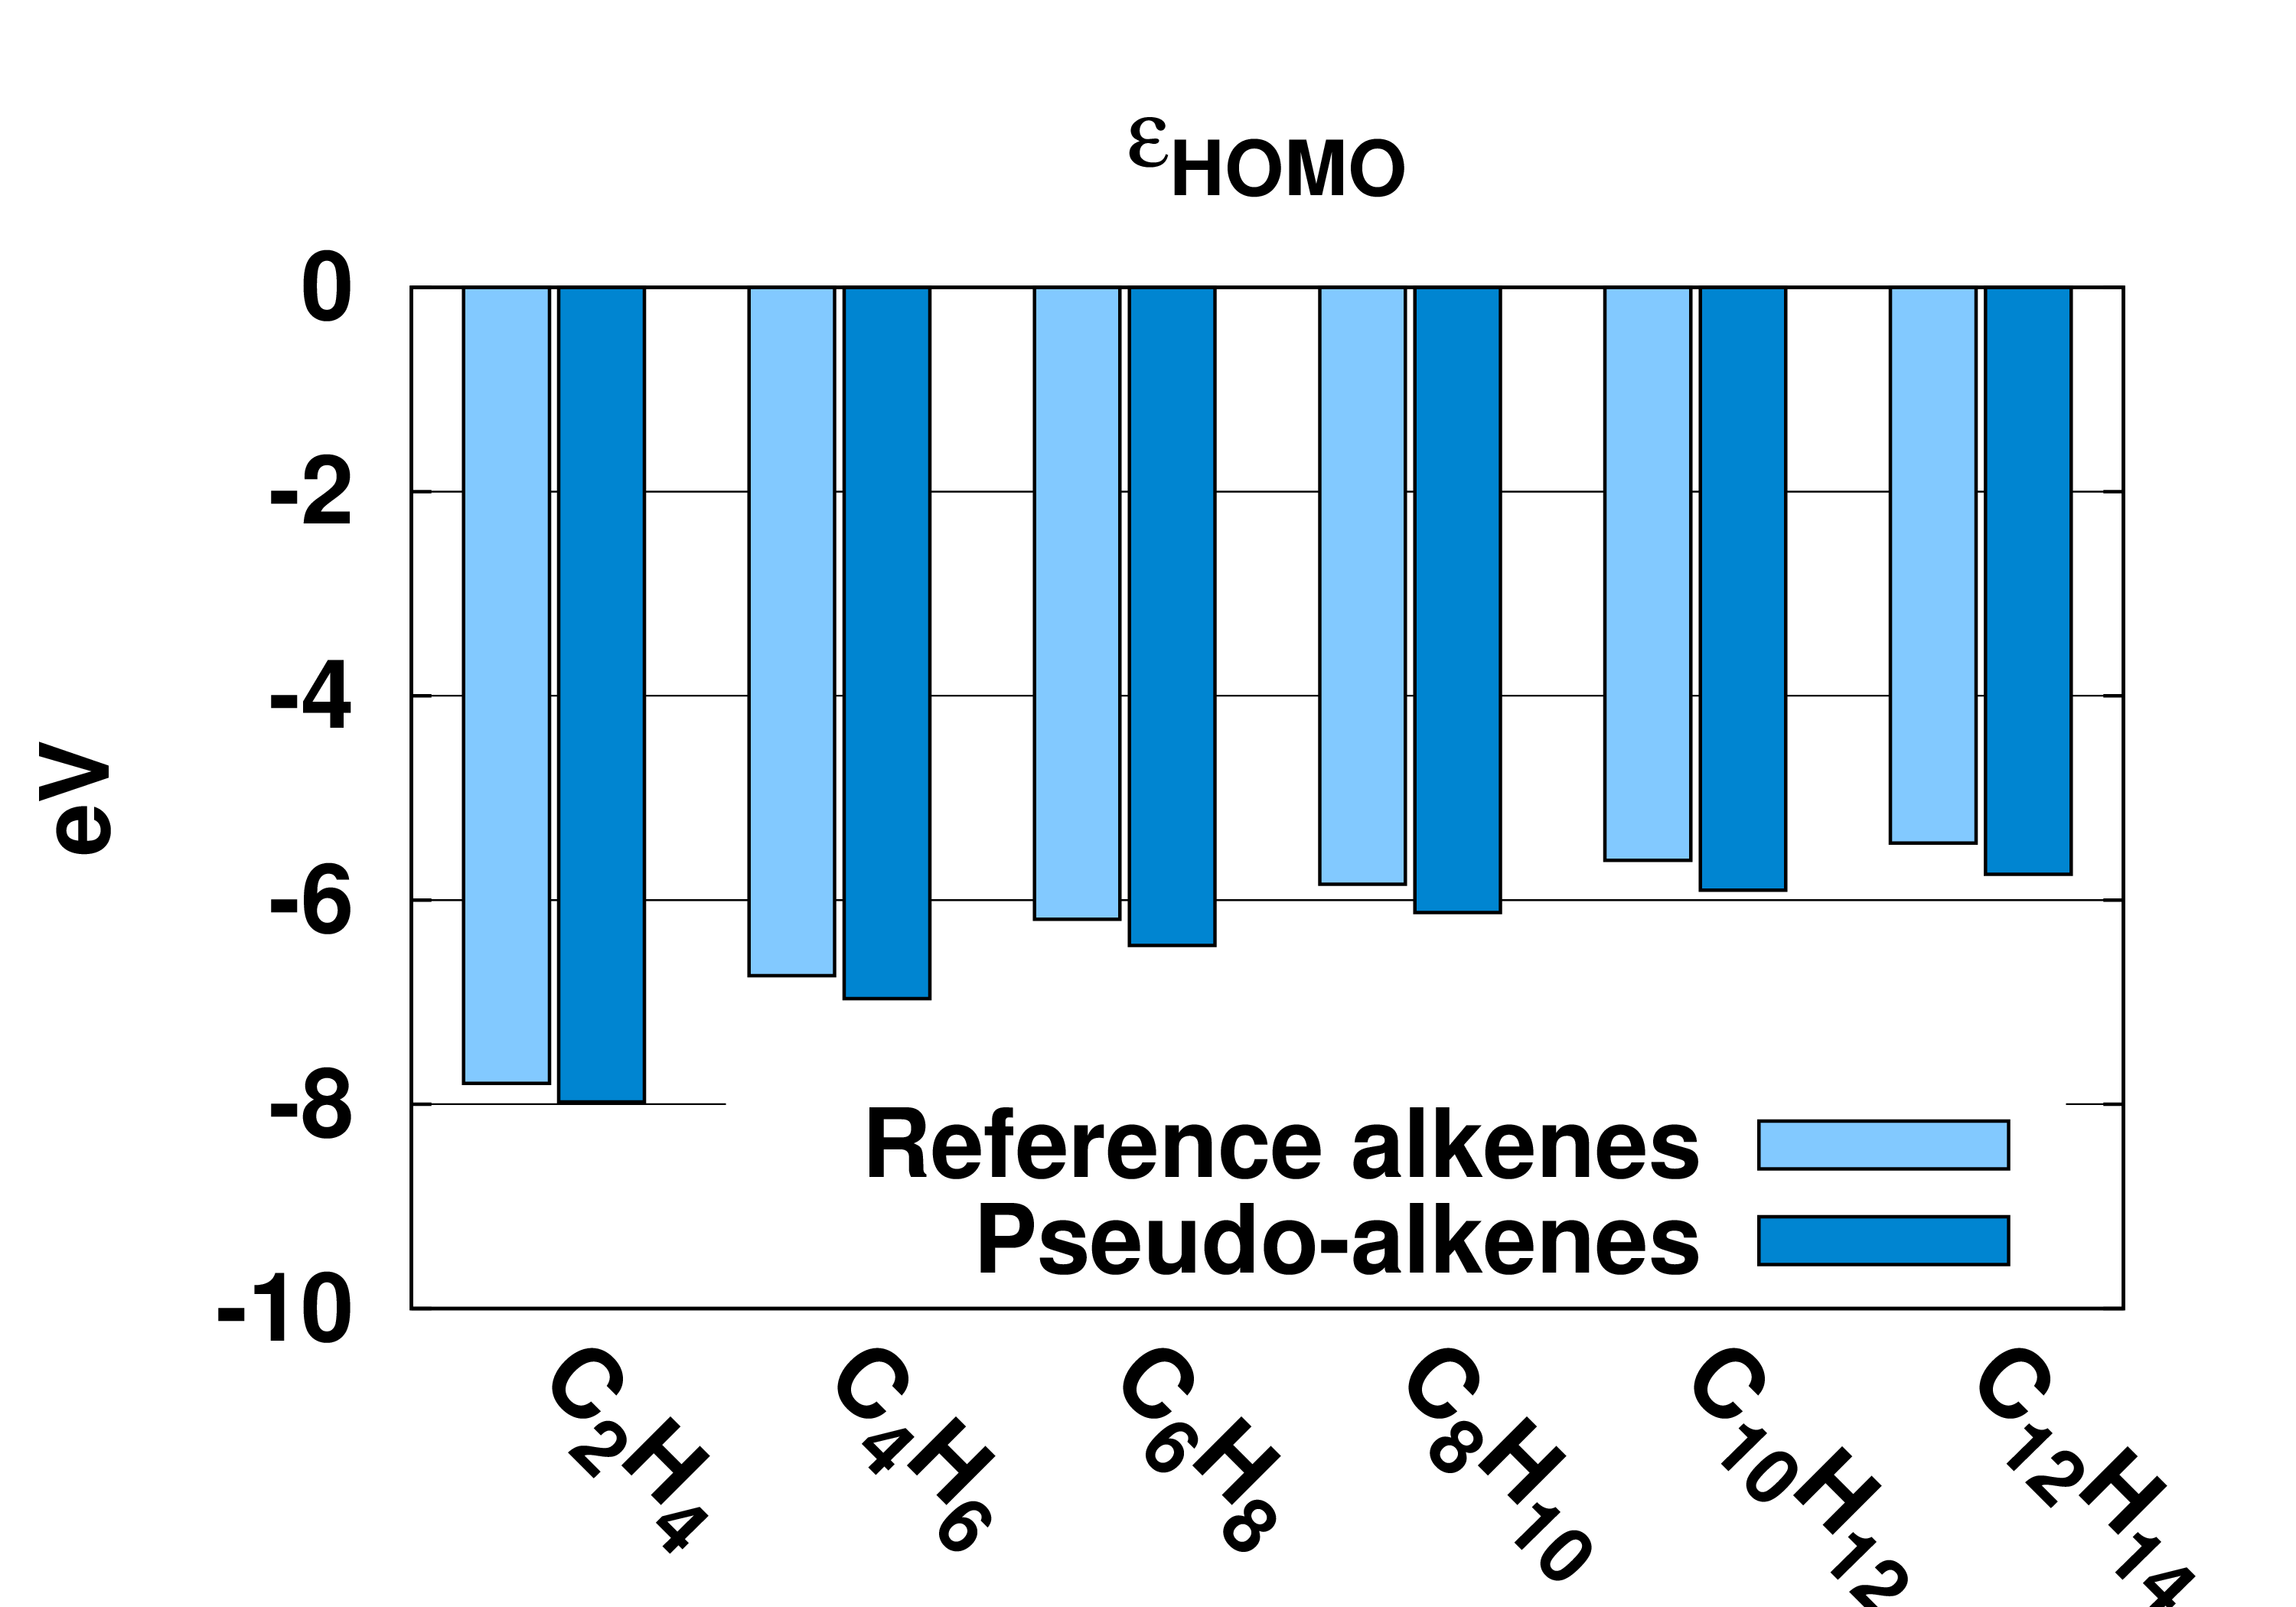
\includegraphics[width=7cm]{short_pbe0_homo}
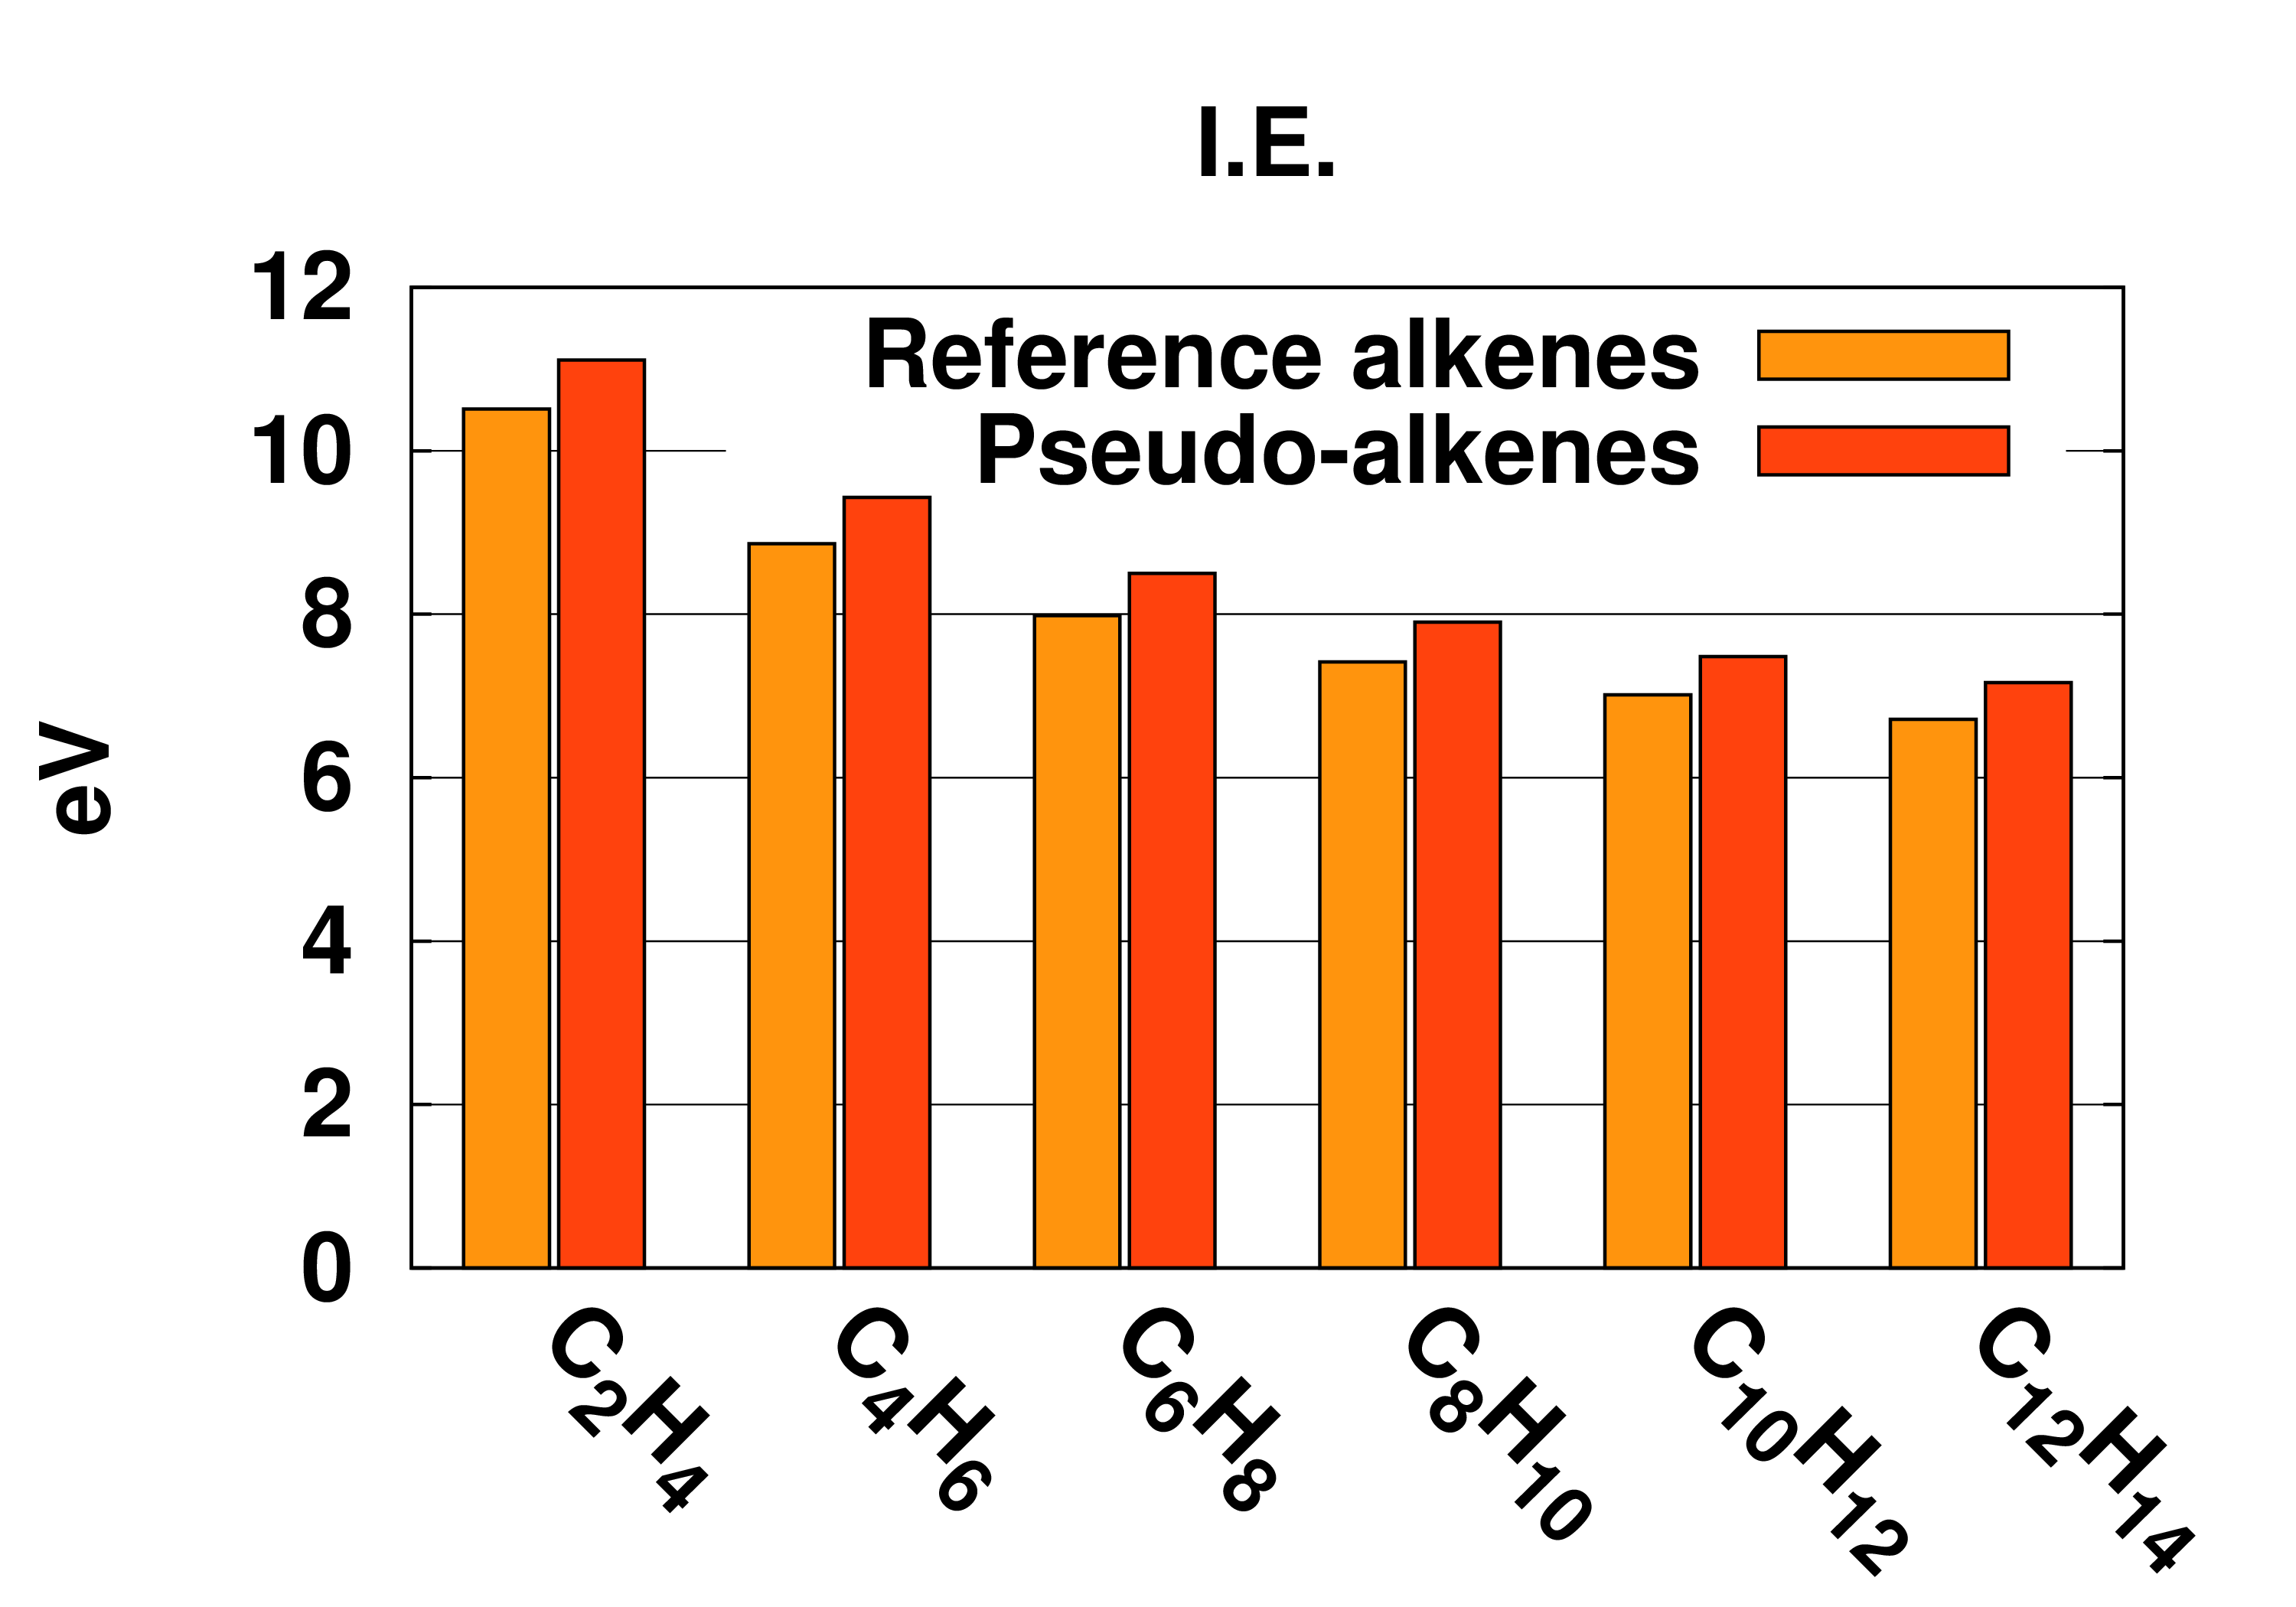
\includegraphics[width=7cm]{short_pbe0_ie}
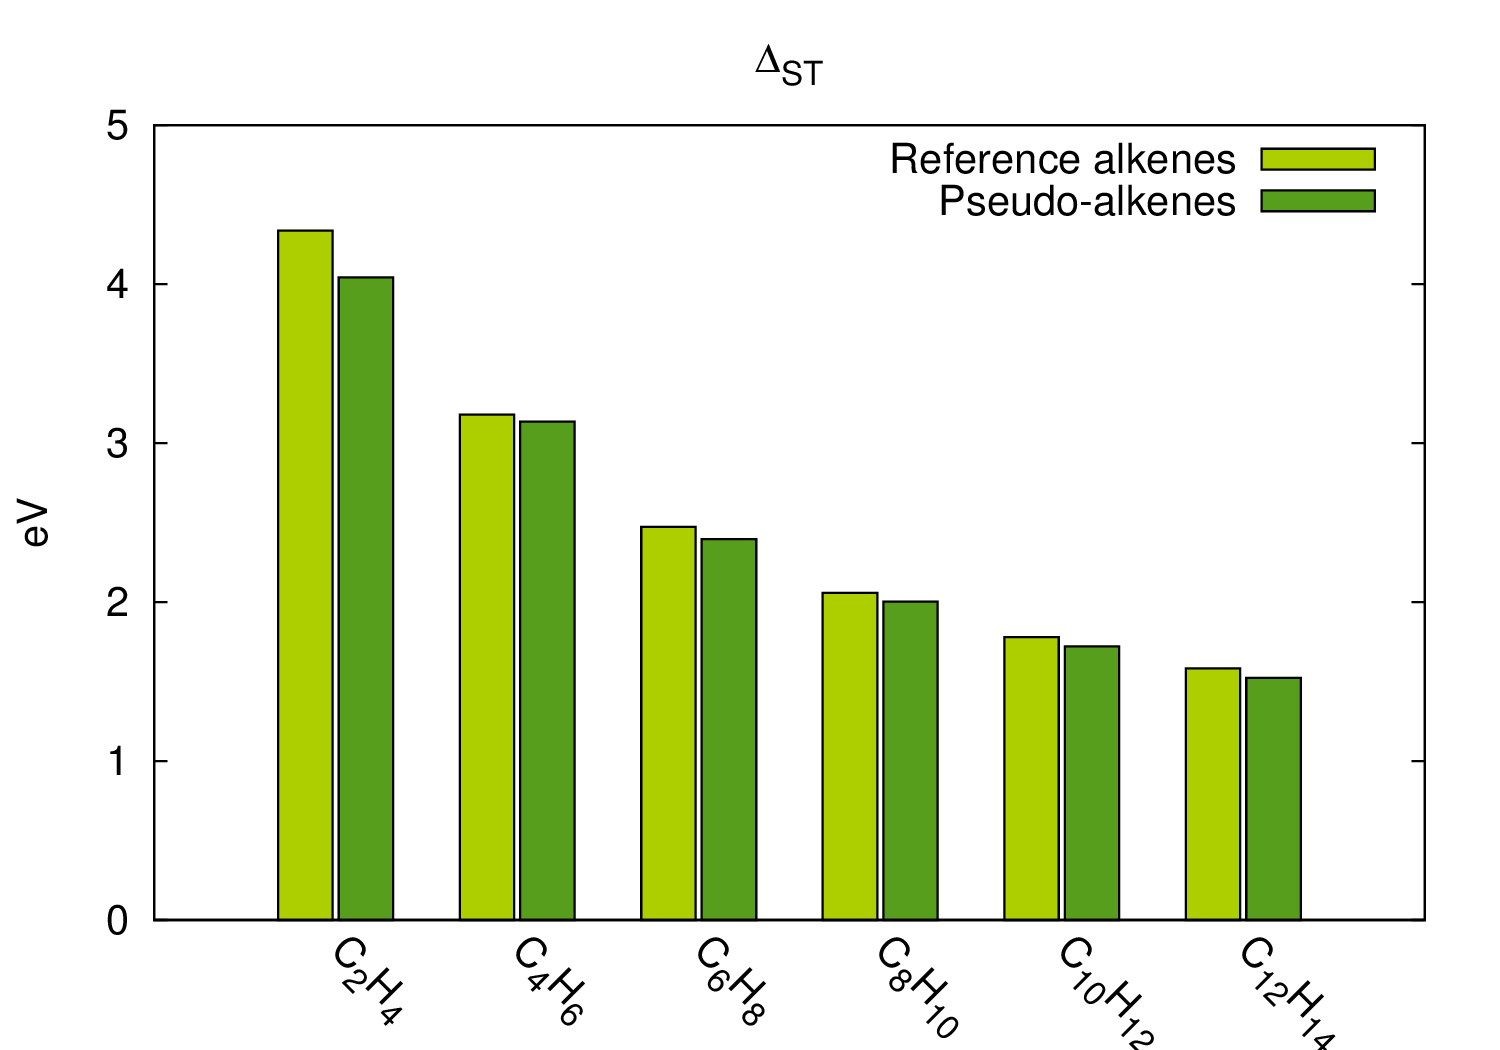
\includegraphics[width=7cm]{short_pbe0_st}
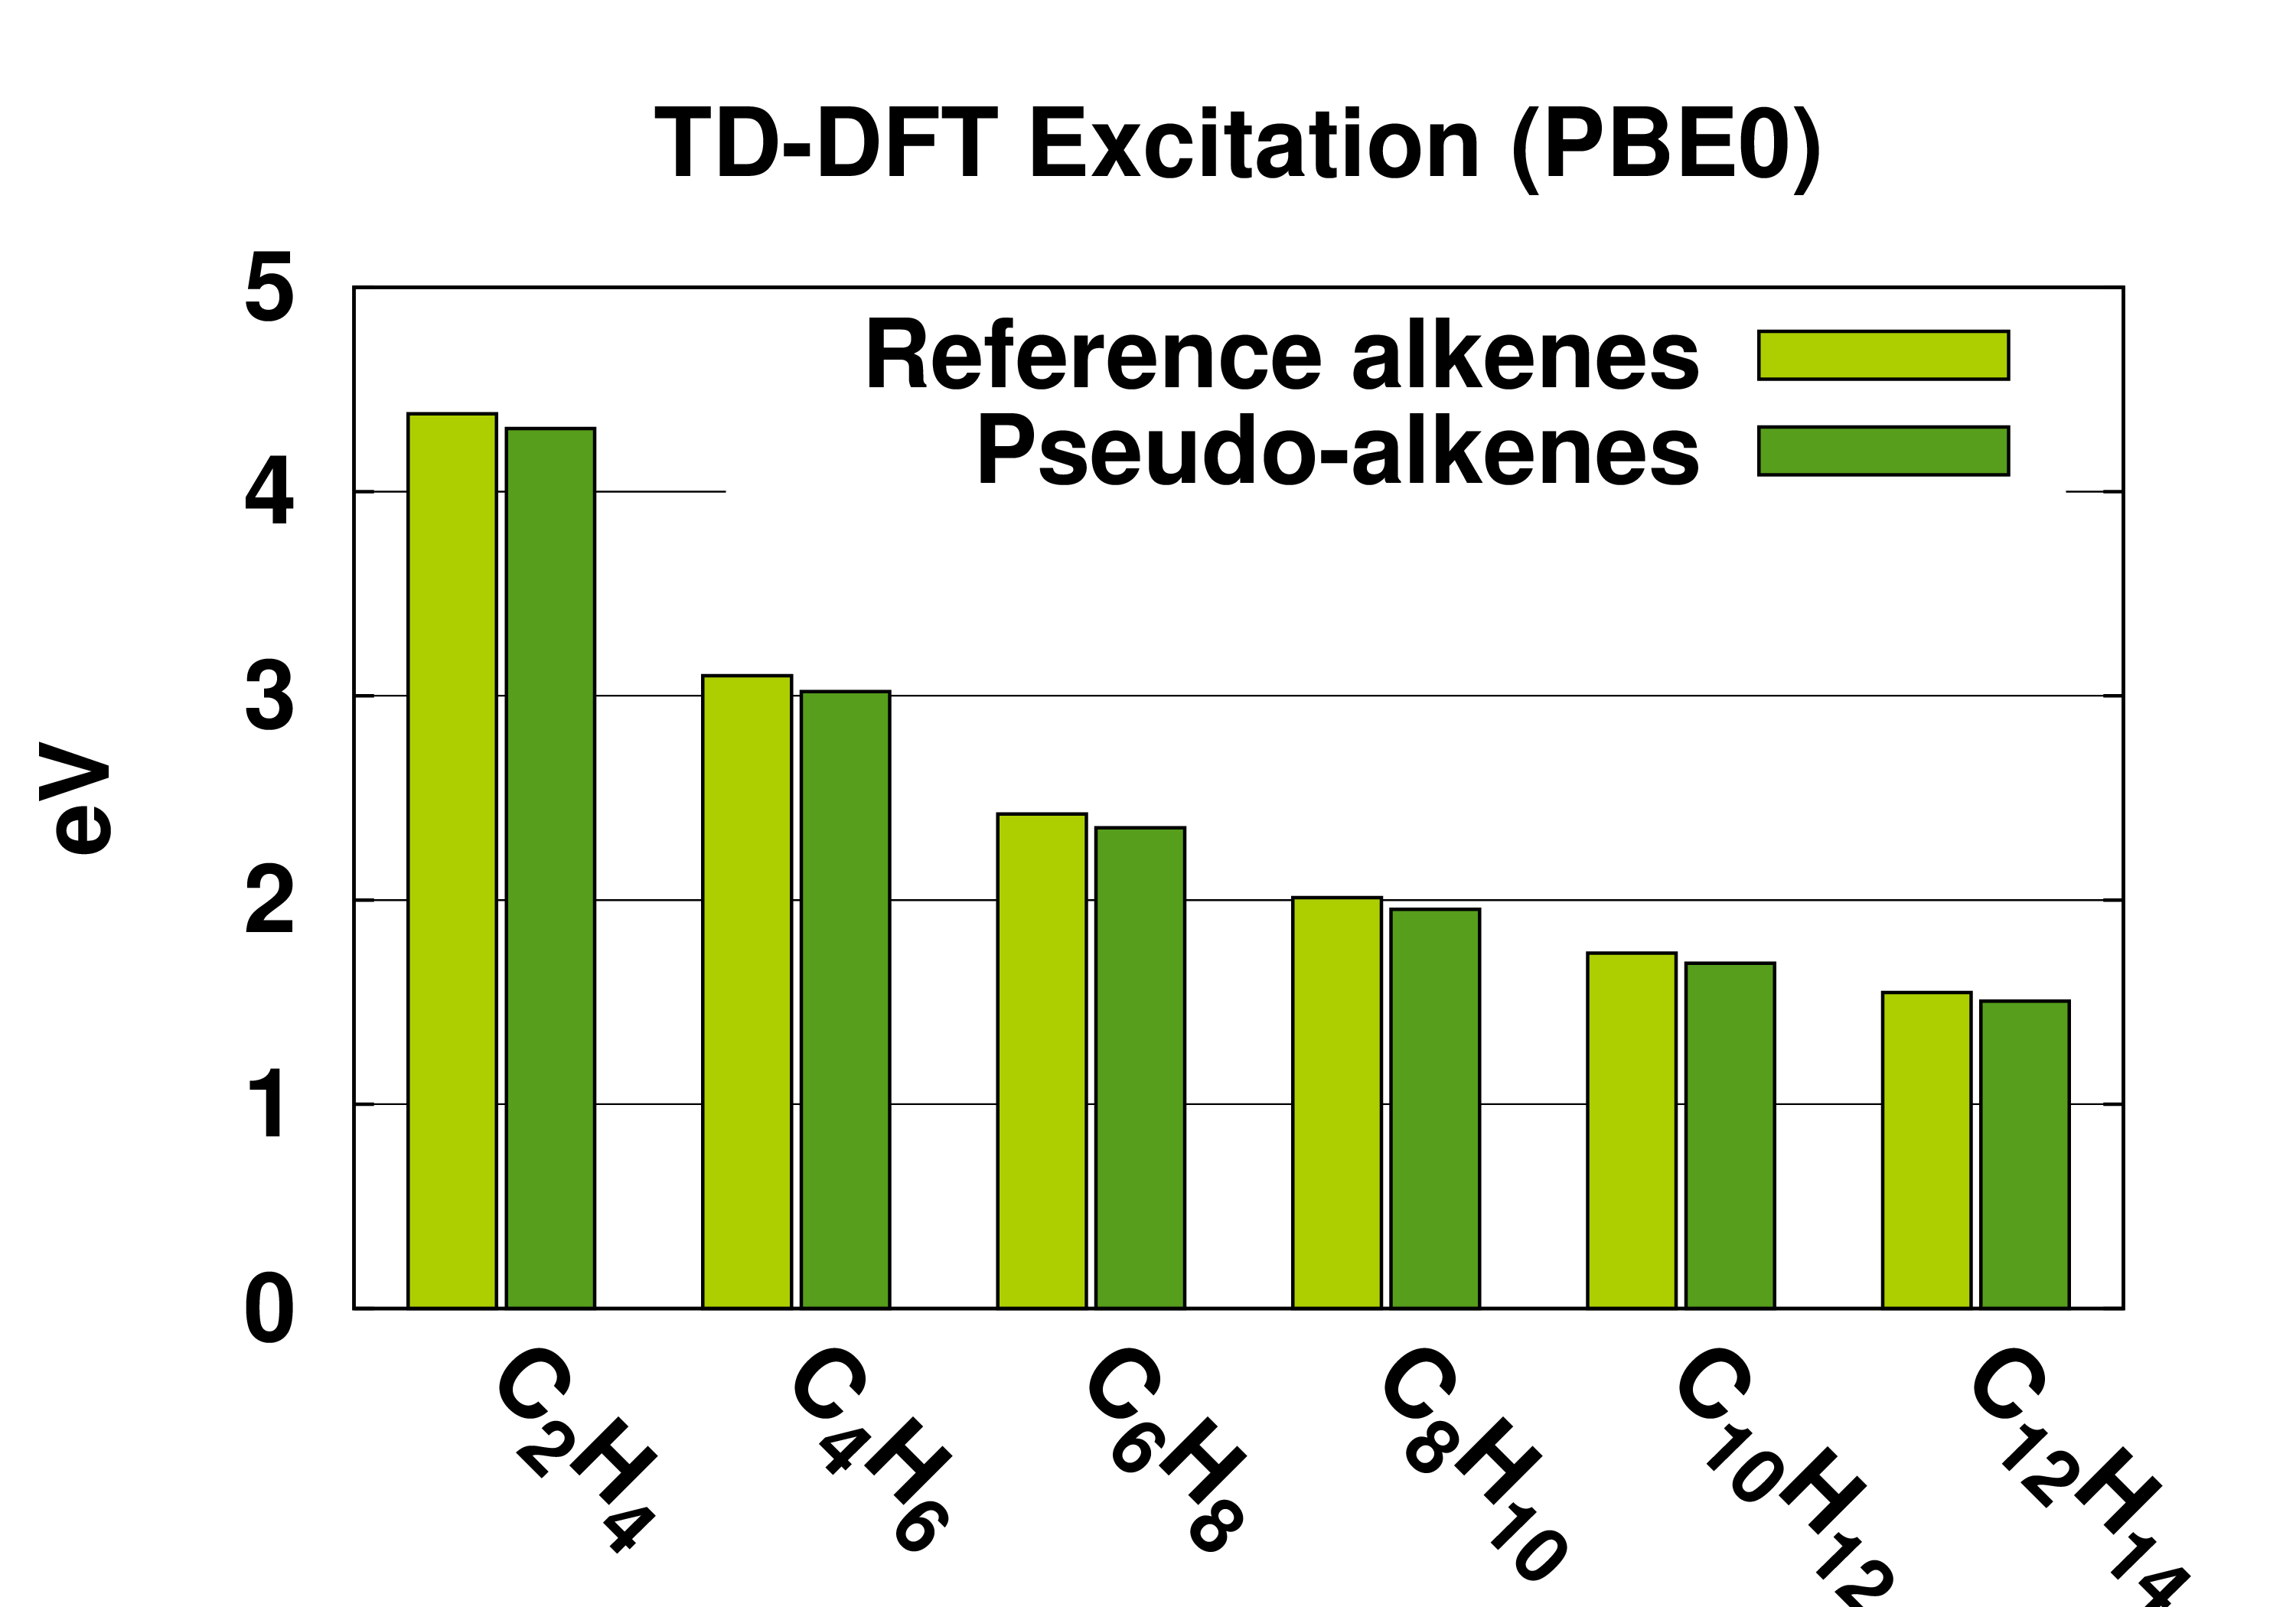
\includegraphics[width=7cm]{short_pbe0_tddft}
\end{center}
\caption{Comparison of the HOMO ($\varepsilon_{HOMO}$),
the ionisation (I.E.), and
the first singlet-triplet $\pi-\pi^*$ excitation ($\Delta_{ST}$ and TD-DFT) energies
between the
all-electron reference and optimal pseudo-potential systems across a range of chain alkenes.
The $\Delta_{ST}$ values are the difference
between the lowest $\pi^*$ triplet (unrestricted formalism) and the lowest singlet state
(restricted formalism).
Calculations are at the PBE0/def-SV(P) level.}
\label{fig:alkenes_pbe0_dft}
\end{figure}

\begin{table}[ht]
\caption{Mean relative errors (in percent) across methods (HF or different functionals)
for short chain alkenes  (C\(_{2}\)-C\(_{12}\)).
The basis set is def-SV(P).}
\begin{tabular}{l r r r r r }
\hline \hline
\%-error                & HF & PBE0 & PBE & TPSS & TPSSh \\
\hline
$\varepsilon_{HOMO}$    & 1.3 & 4.0 & 8.5 & 12.0 &  9.7 \\
I.E.                    & 5.3 & 6.0 & 8.1 & 10.1 &  9.0 \\
$\Delta_{ST}$           & 4.1 & 3.6 & 7.5 & 13.3 & 11.4 \\
TD-DFT $\pi-\pi^*$       & 11.6 & 2.6 & 2.8 &  6.3 &  6.9 \\ 
\hline\hline
\end{tabular}
\label{table:alkene_errors}
\end{table}

Also compared are TD-DFT results for this system and results of some of the authors' previous work,
which match to within 3\% (see supplementary materials).\cite{drujon_pseudopotentials_2013}
%Let us recall here that in our previous work potentials were placed at the center of bonds.

Here we discuss in more detail the results obtained with the PBE0 functional presented
in Figure~\ref{fig:alkenes_pbe0_dft}.
The properties computed with the optimal pseudo-potential are in very close agreement with the reference values.
%The HOMO energy and the ionisation energy are quantities very difficult to reproduce
%owing to the fact that the atomic charges of the pseudo-atoms were drastically modified.
Even for HOMO and ionisation energies, the agreement between pseudo and reference calculations is satisfactory
(average error $\le 6\%$).
Thus, the addition or withdrawal of an electron from the pseudo-molecule is well reproduced.
Furthermore, the first singlet-triplet $\pi-\pi^*$ excitations agree very well in either
the $\Delta_{ST}$ or TD-DFT framework (average error $\le 3.6\%$).

\subsection{Fused rings and larger chains}

\begin{figure}
\begin{center}
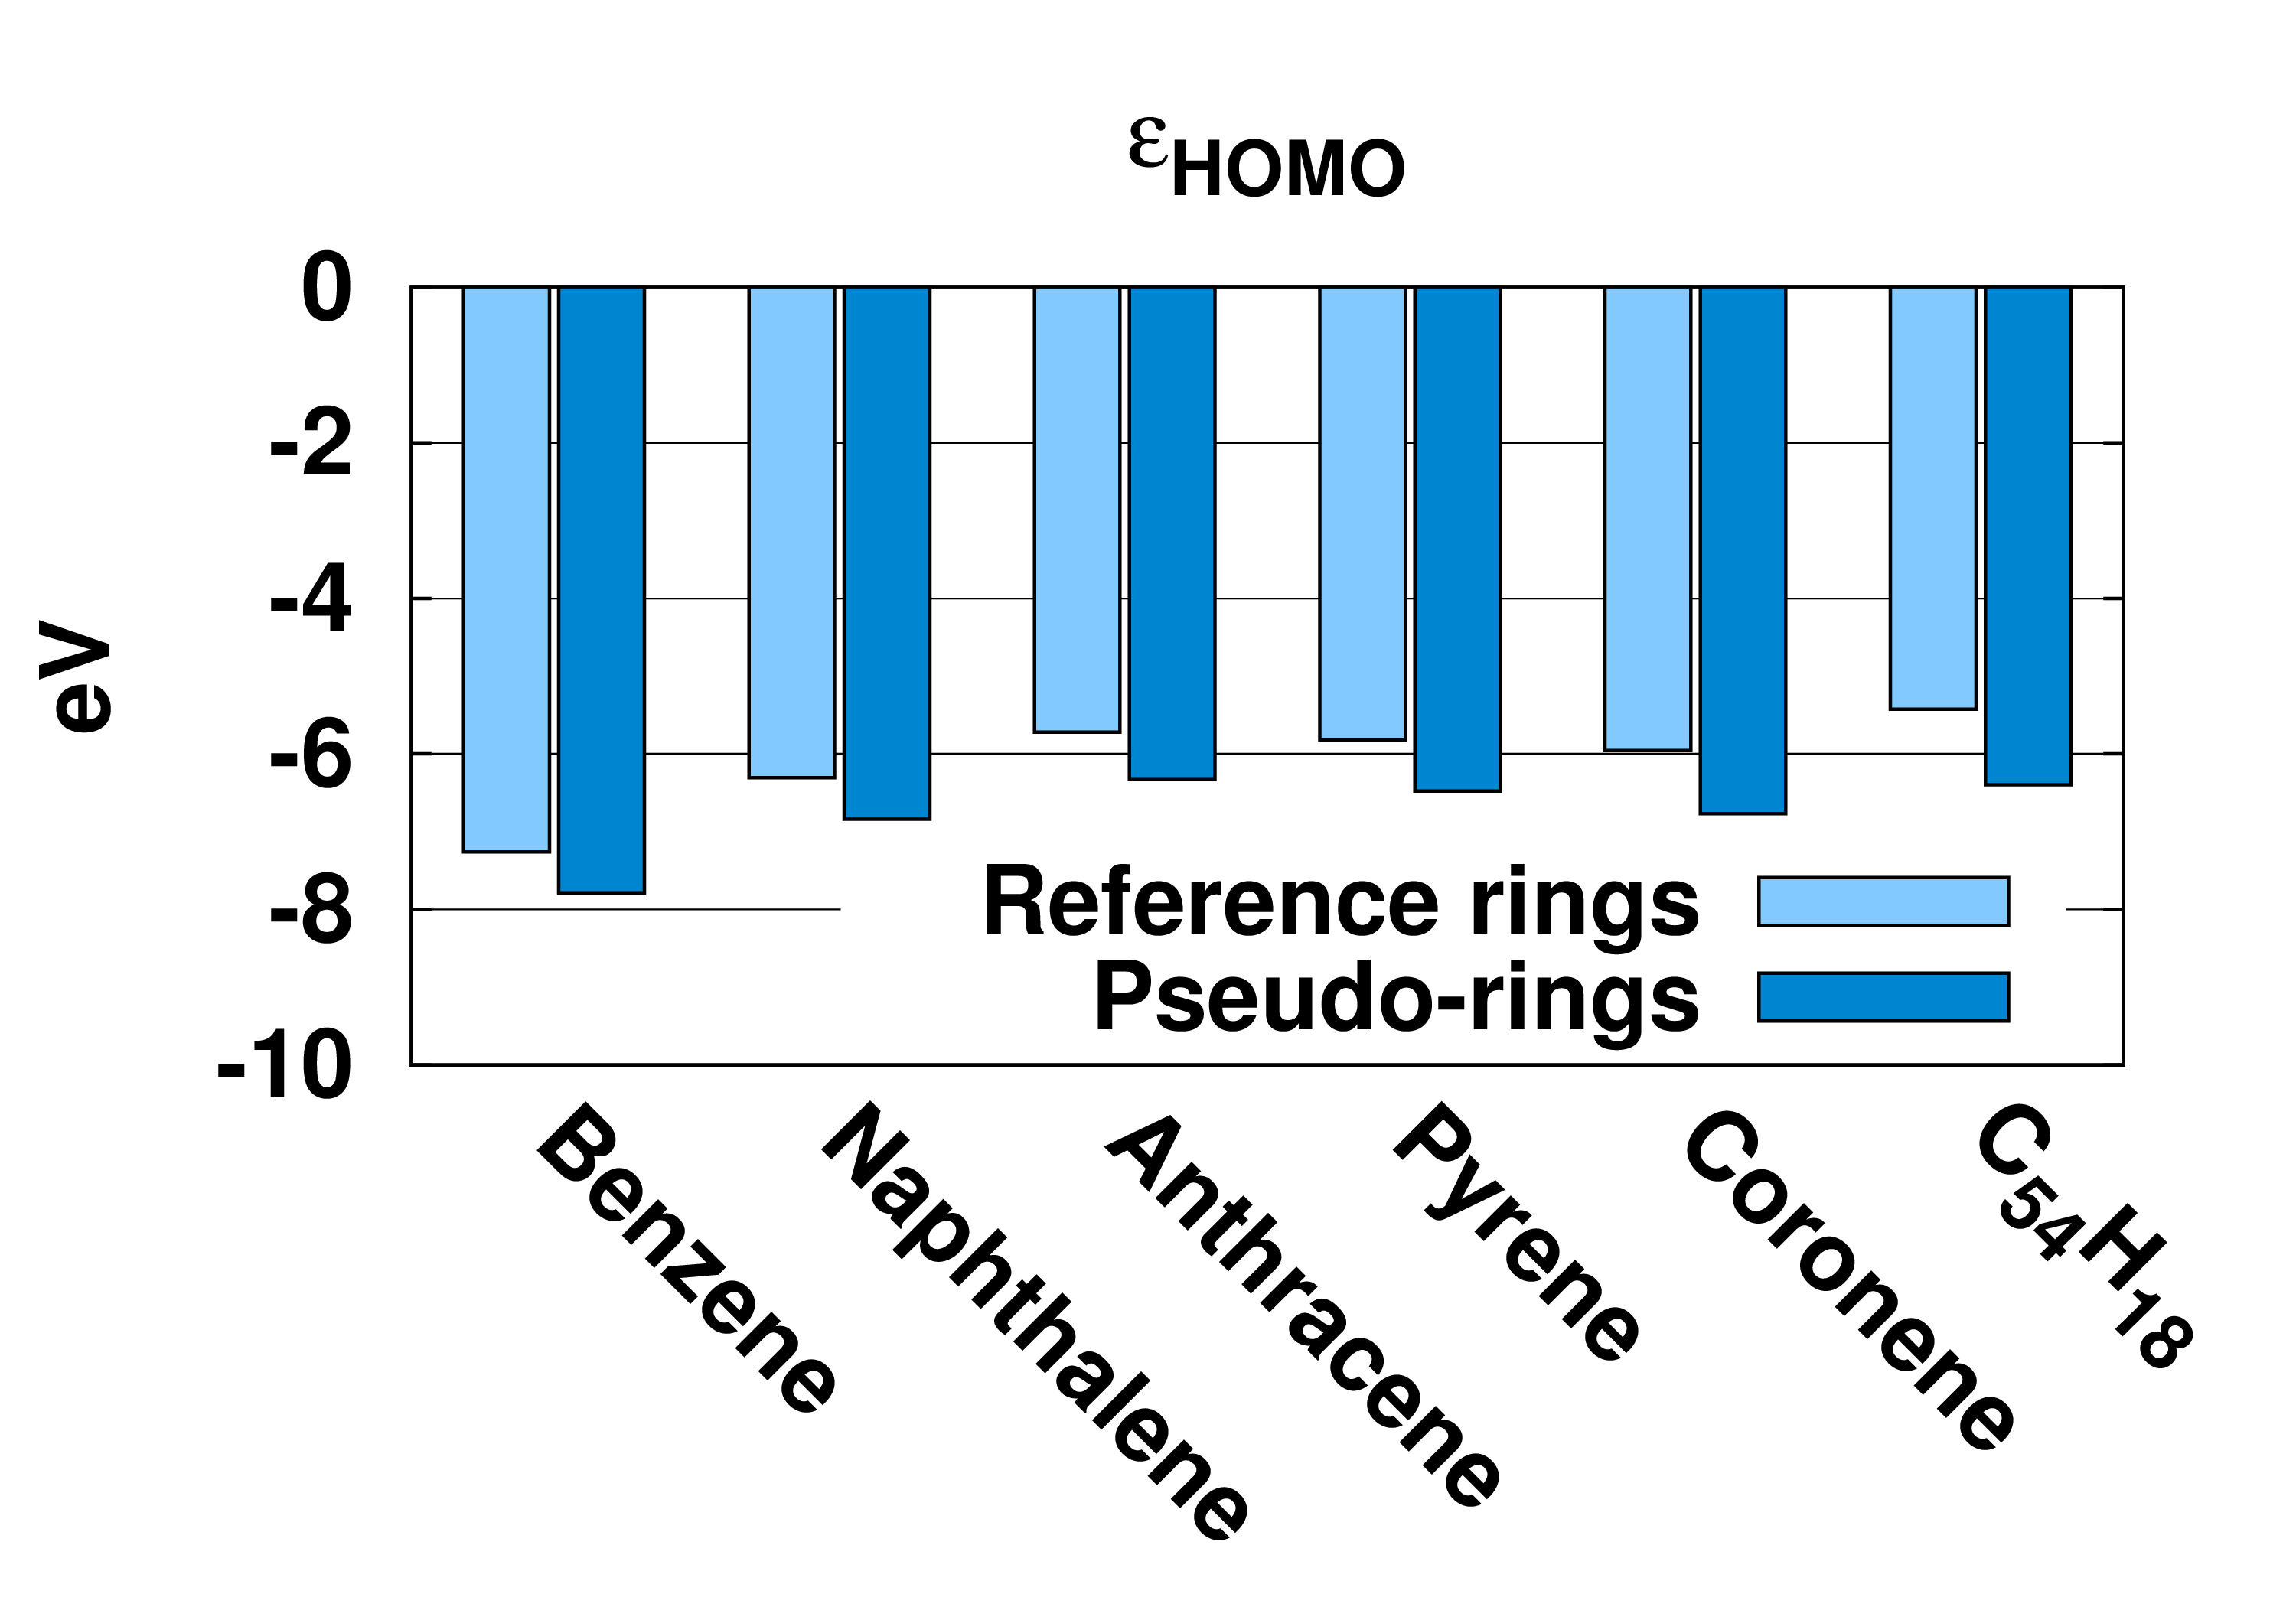
\includegraphics[width=7cm]{ring_pbe0_homo}
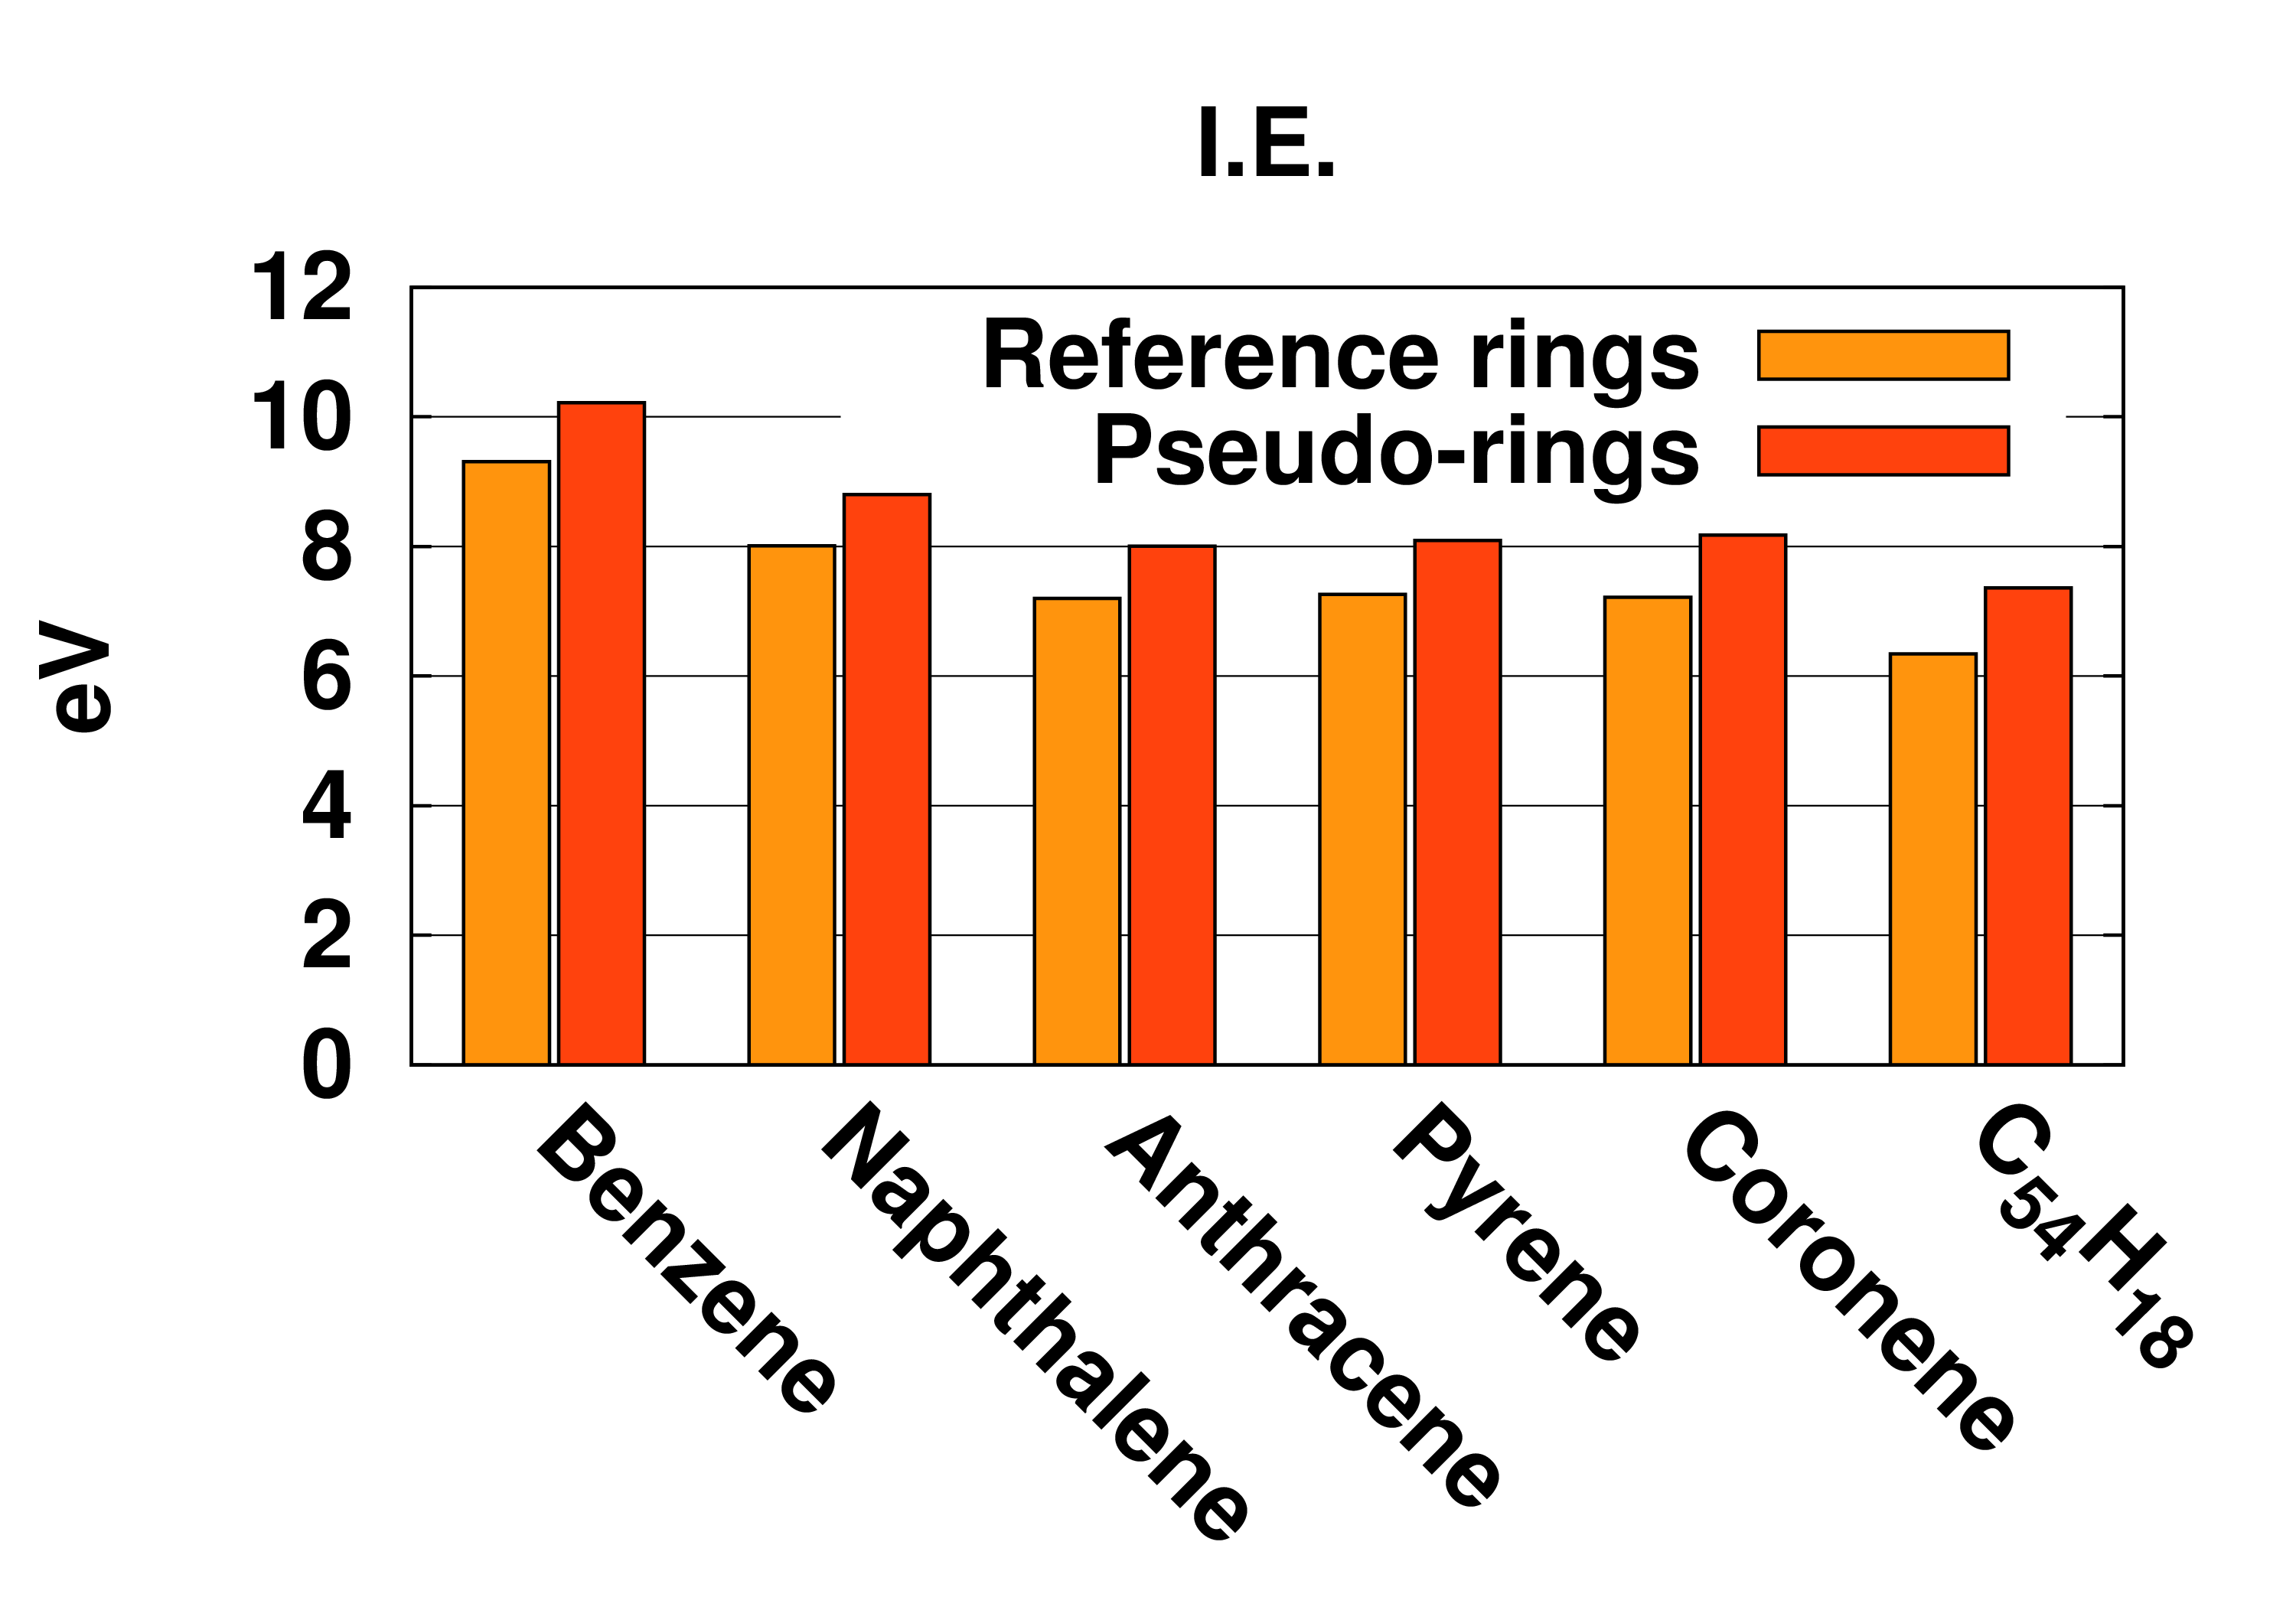
\includegraphics[width=7cm]{ring_pbe0_ie}
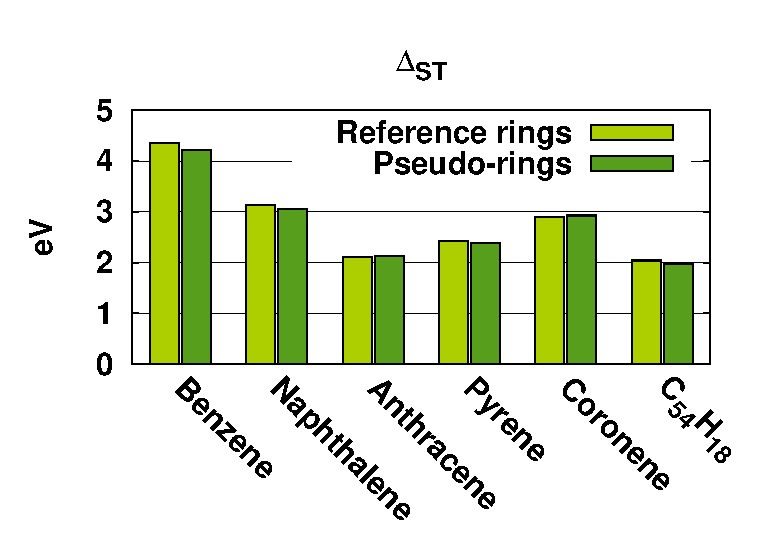
\includegraphics[width=7cm]{ring_pbe0_st}
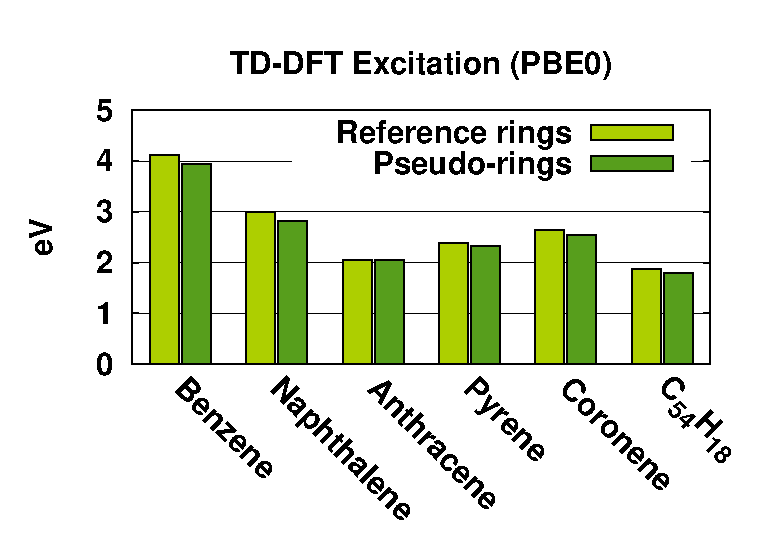
\includegraphics[width=7cm]{ring_pbe0_tddft}
\end{center}
\caption{Comparison of the HOMO ($\varepsilon_{HOMO}$),
the ionisation (I.E.),
the first singlet-triplet $\pi-\pi^*$ excitation ($\Delta_{ST}$ and TD-DFT) energies
between the
all electron reference system and the optimal pseudo-potential across a range of ring molecules.
The $\Delta_{ST}$ values are the difference
between the lowest $\pi^*$ triplet (unrestricted formalism) and the lowest singlet state
(restricted formalism).
Calculations are at the PBE0/def-SV(P) level.
The C\(_{54}\)H\(_{18}\) molecule is represented in Figure \ref{fig:c54h18}.}
\label{fig:rings_graphs}
\end{figure}

\begin{figure}
\begin{center}
\fbox{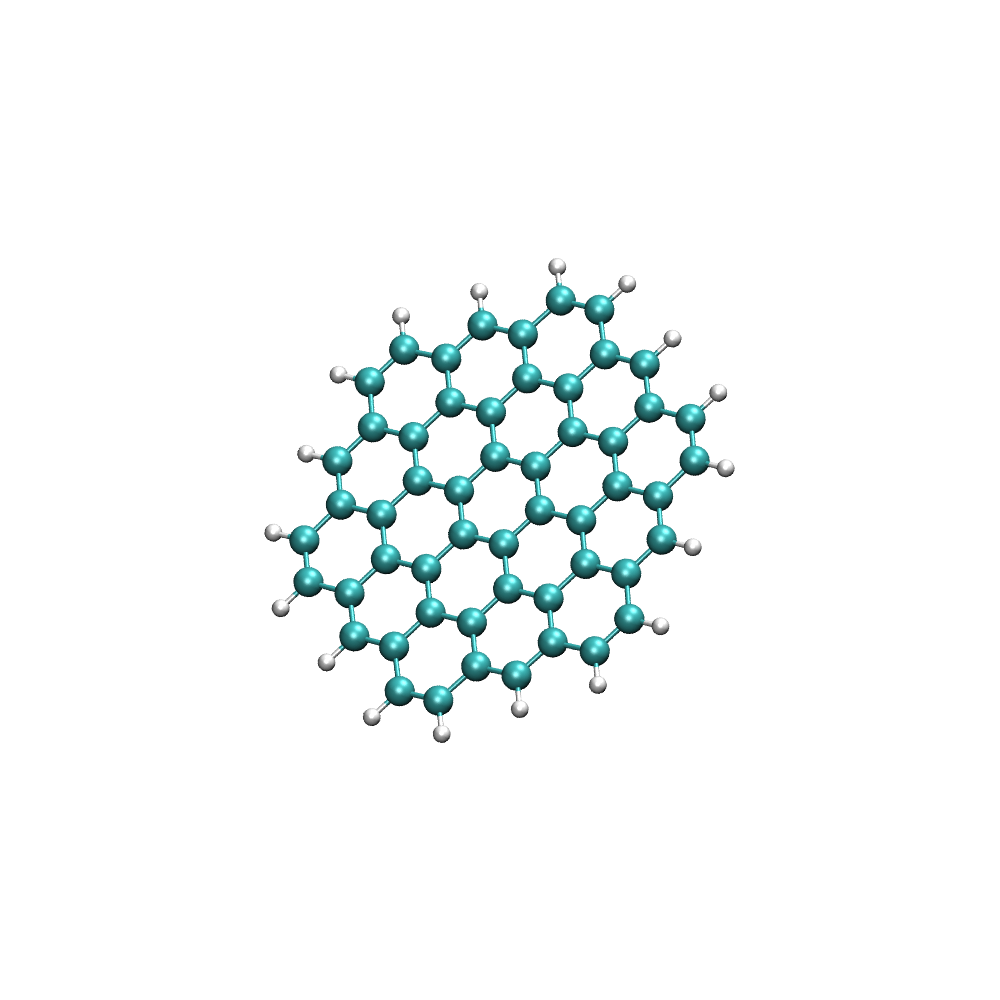
\includegraphics[width=5cm]{c54h18}}
\end{center}
\caption{\label{fig:c54h18}The C\(_{54}\)H\(_{18}\) molecule.}
\end{figure}

The potentials derived above are also tested on larger systems.
Figure \ref{fig:rings_graphs} shows the $\Delta_{ST}$, the IE and
HOMO energy values for several ring systems, the largest of which is C$_{54}$H$_{18}$, shown in Figure~\ref{fig:c54h18}.
As with the short chain alkenes, the general trend of the results is well-replicated
by the pseudo-systems, and the percentage errors, displayed in Table
\ref{table:ring_system_errors}, are similar. For PBE0, Figure~\ref{fig:rings_graphs}, mean average errors are below 3.6\% for excitation energies, independently of the way they are computed
($\Delta_{ST}$ or TD-DFT). For HOMO and ionisation energies, average errors are somewhat larger, up to 10\%. 
%In the case of ionisation, the loss of aromaticity due to the %variation of the number of
%electrons leads to larger discrepancies.
Yet, the agreement between reference and pseudo-potential calculations is very good.
The modeling through our pseudo-potential does not suffer from error accumulation: different pseudo-systems, whether of 2 or 54 pseudo-atoms, lead to similar errors on the computed properties.

\begin{table}[ht]
\caption{Mean relative errors (in percent) across methods (HF or different functionals)
for ring-systems.
The basis set is def-SV(P).}
\begin{tabular}{l r r r r r }
\hline\hline
\%-error                & HF & PBE0 & PBE & TPSS & TPSSh \\
\hline
$\varepsilon_{HOMO}$    & 3.4 &  9.3  & 13.4 & 17.1 & 14.7 \\
I.E.                    & 7.4 & 10.0  & 12.5 & 14.4 & 13.0 \\
$\Delta_{ST}$           & 3.3 &  1.9  &  1.7 &  6.8 &  6.7 \\
TD-DFT $\pi-\pi^*$       & 13.5 &  3.6  &  2.7 &  6.3 &  7.0 \\ 
\hline\hline
\end{tabular}
\label{table:ring_system_errors}
\end{table}

\begin{figure}
\begin{center}
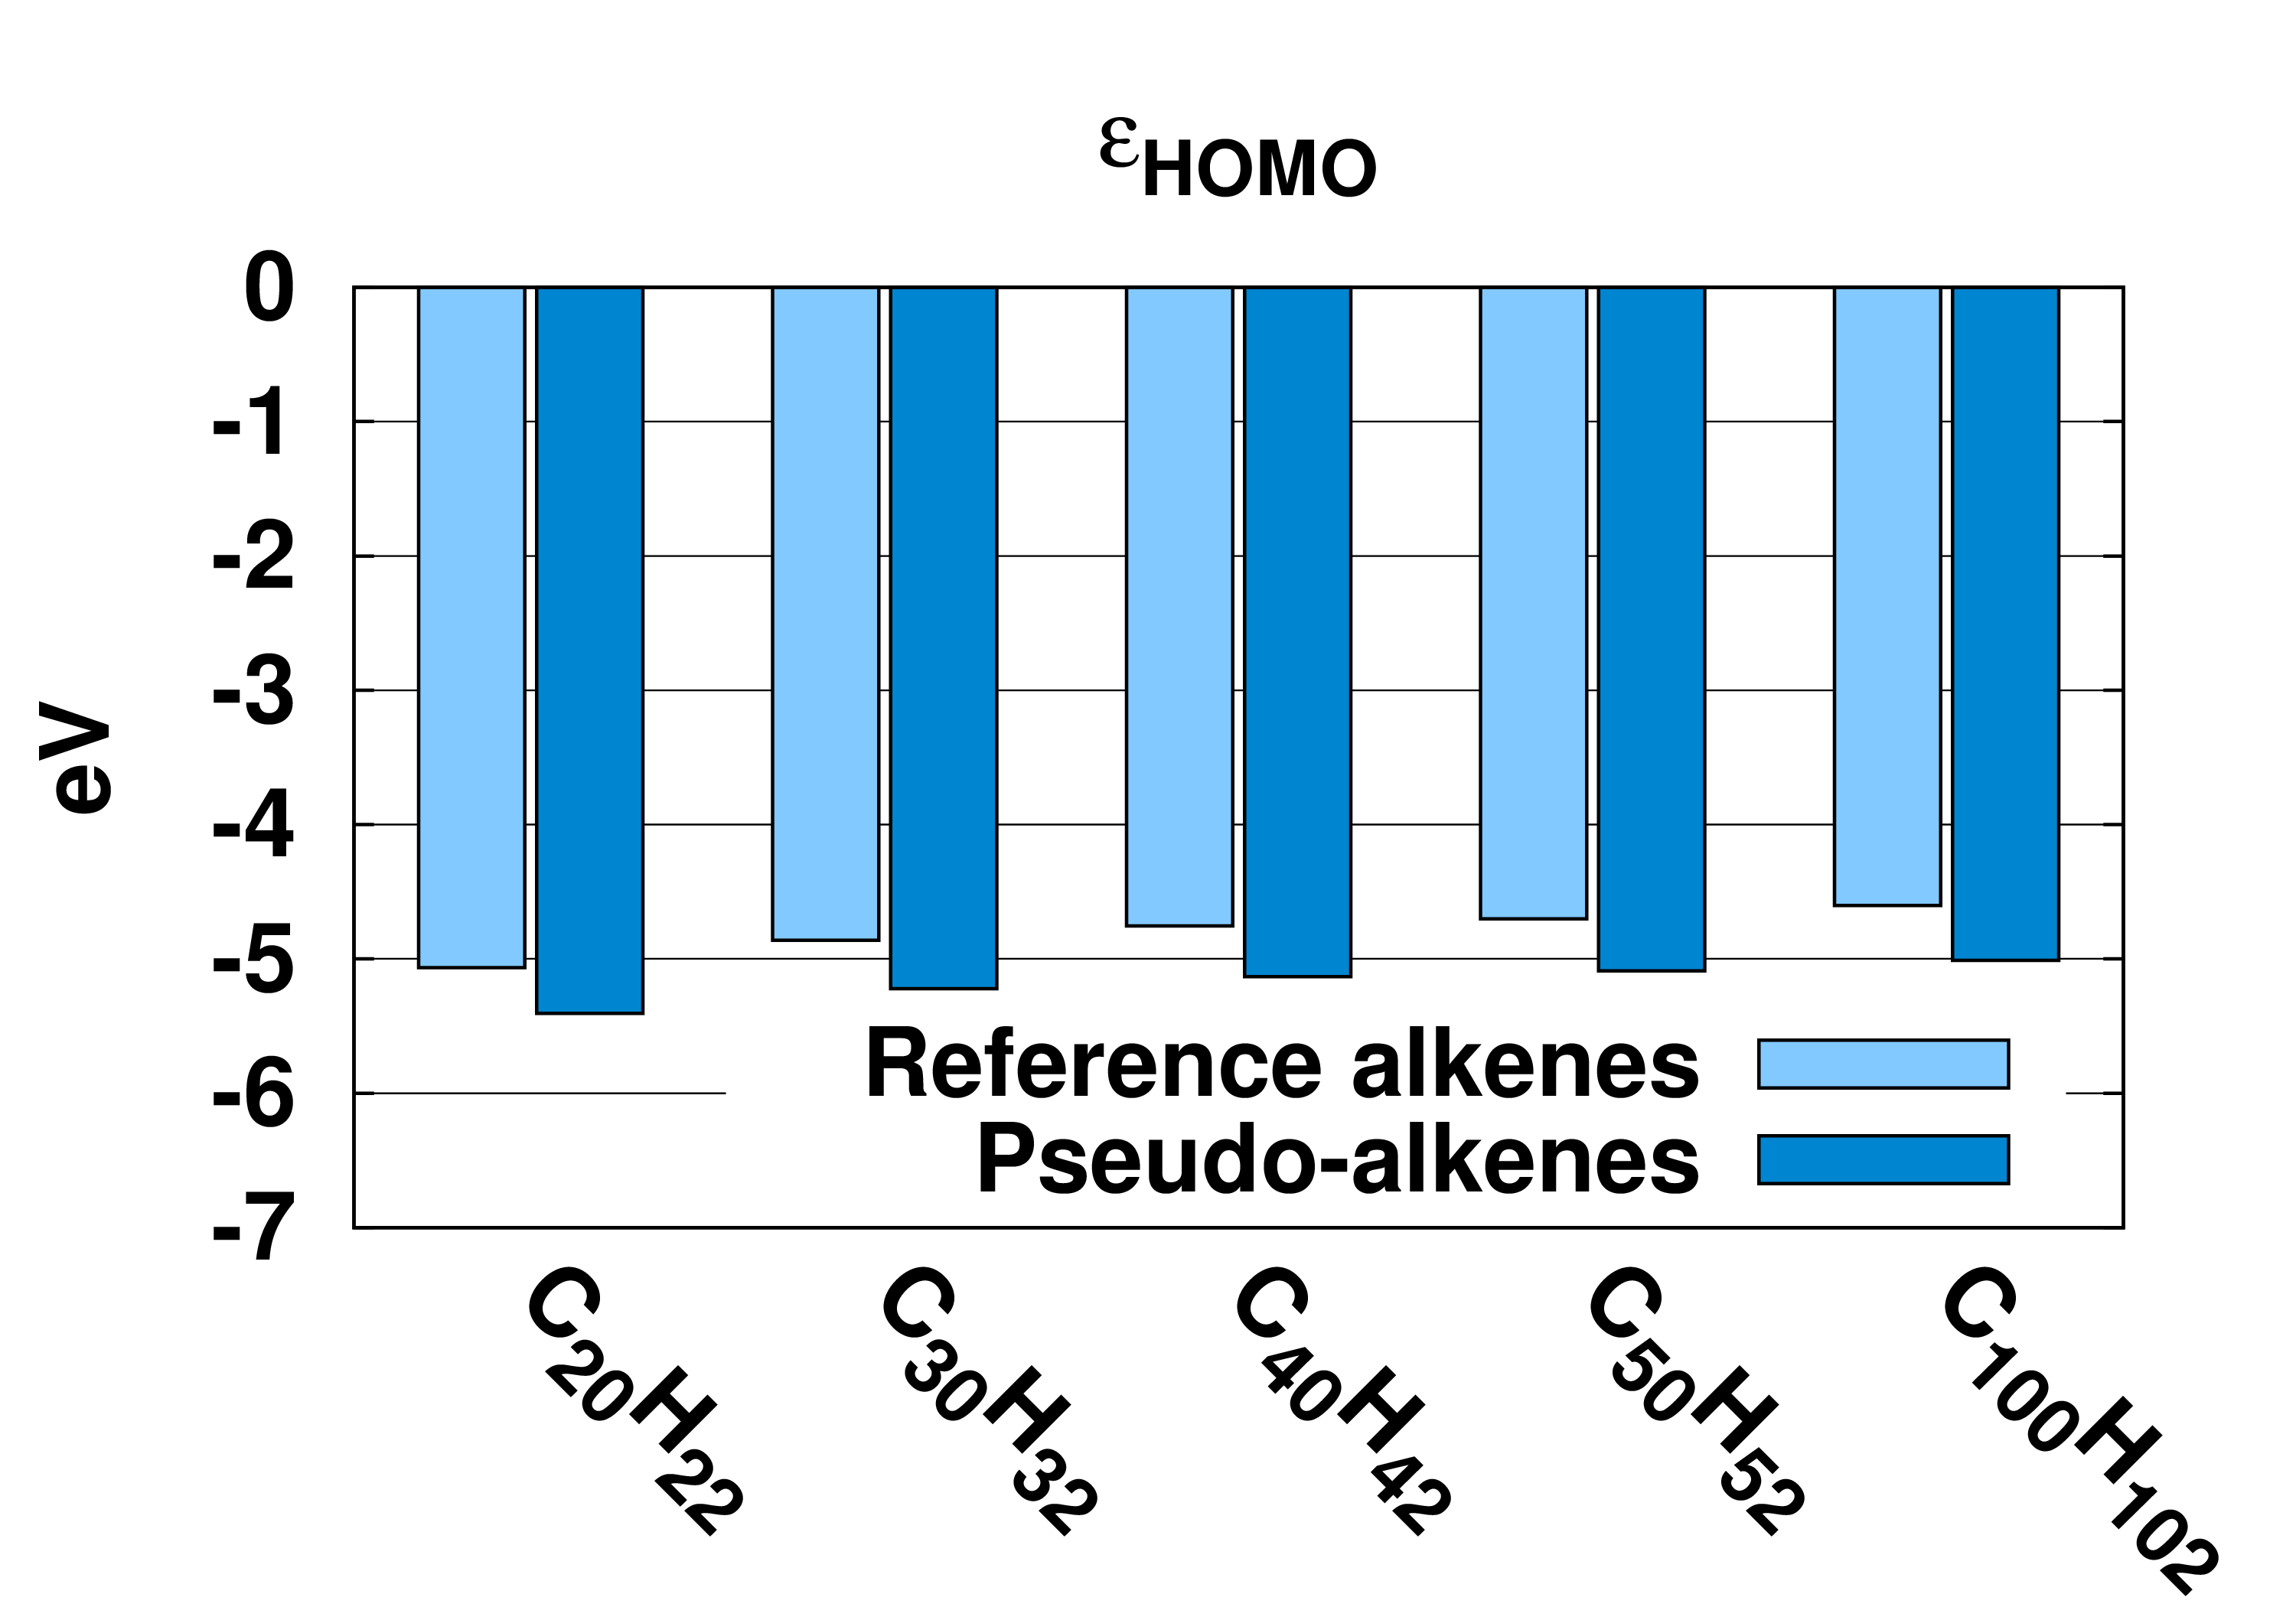
\includegraphics[width=7cm]{long_pbe0_homo}
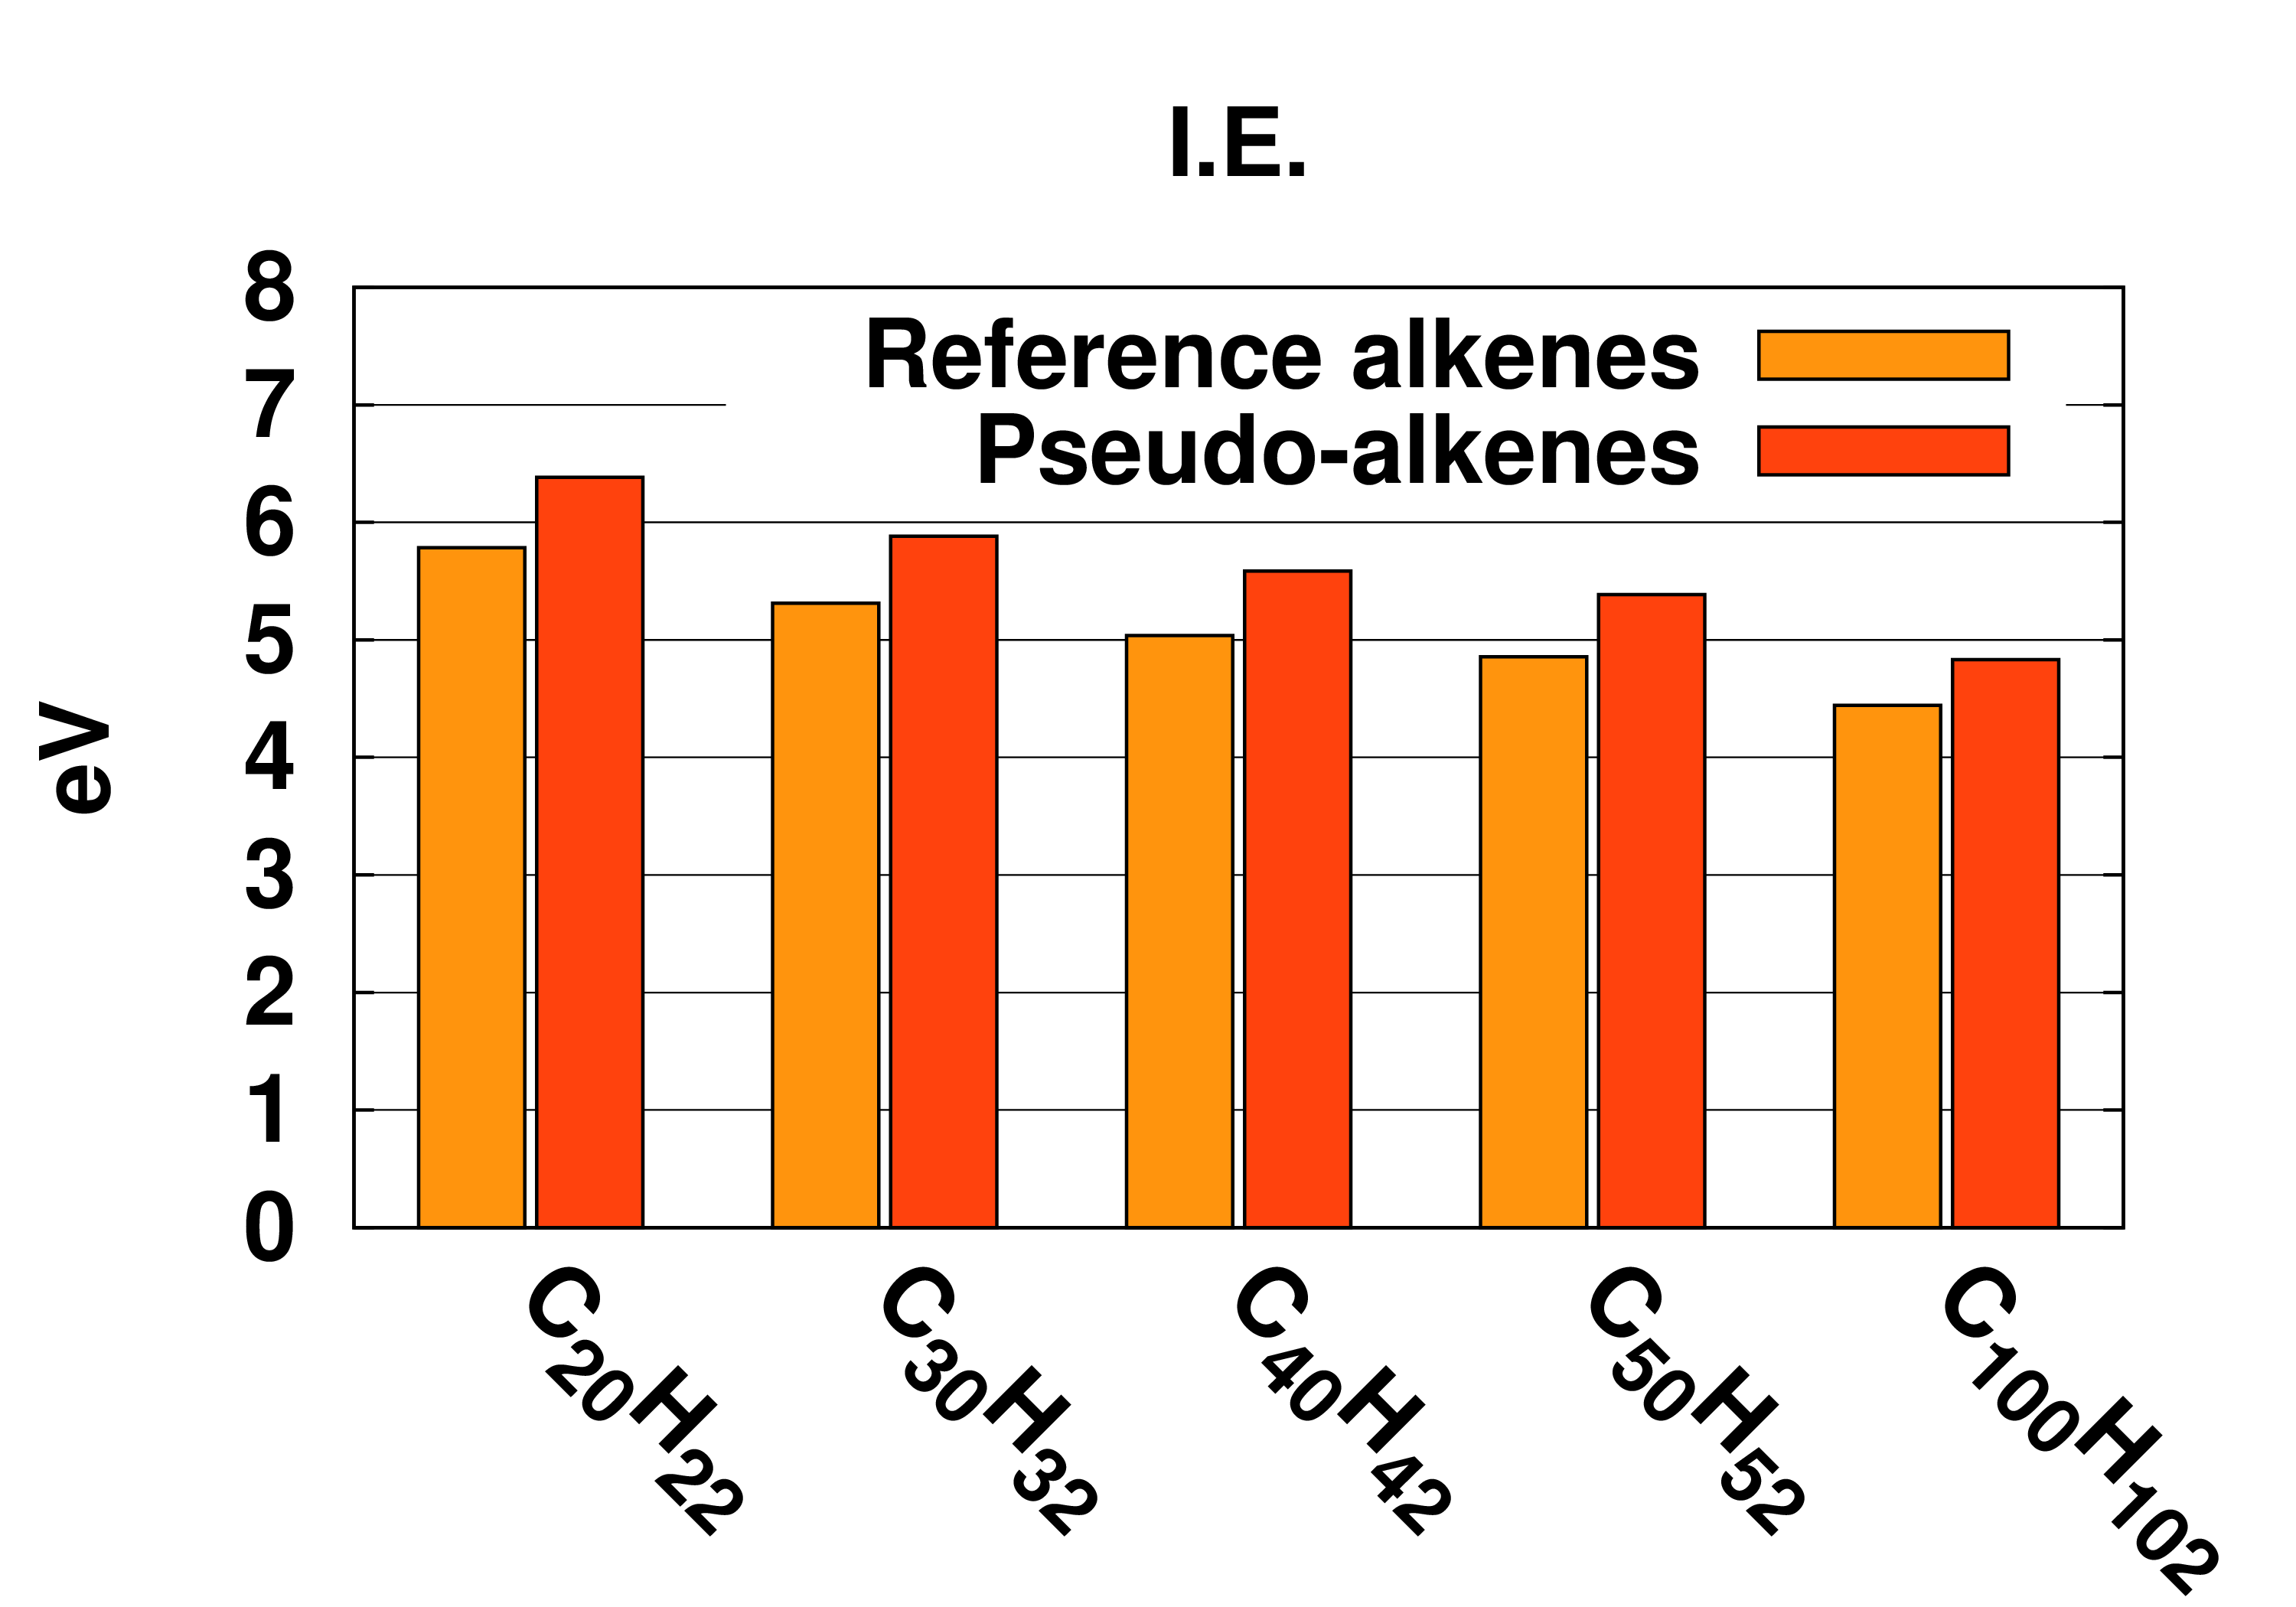
\includegraphics[width=7cm]{long_pbe0_ie}
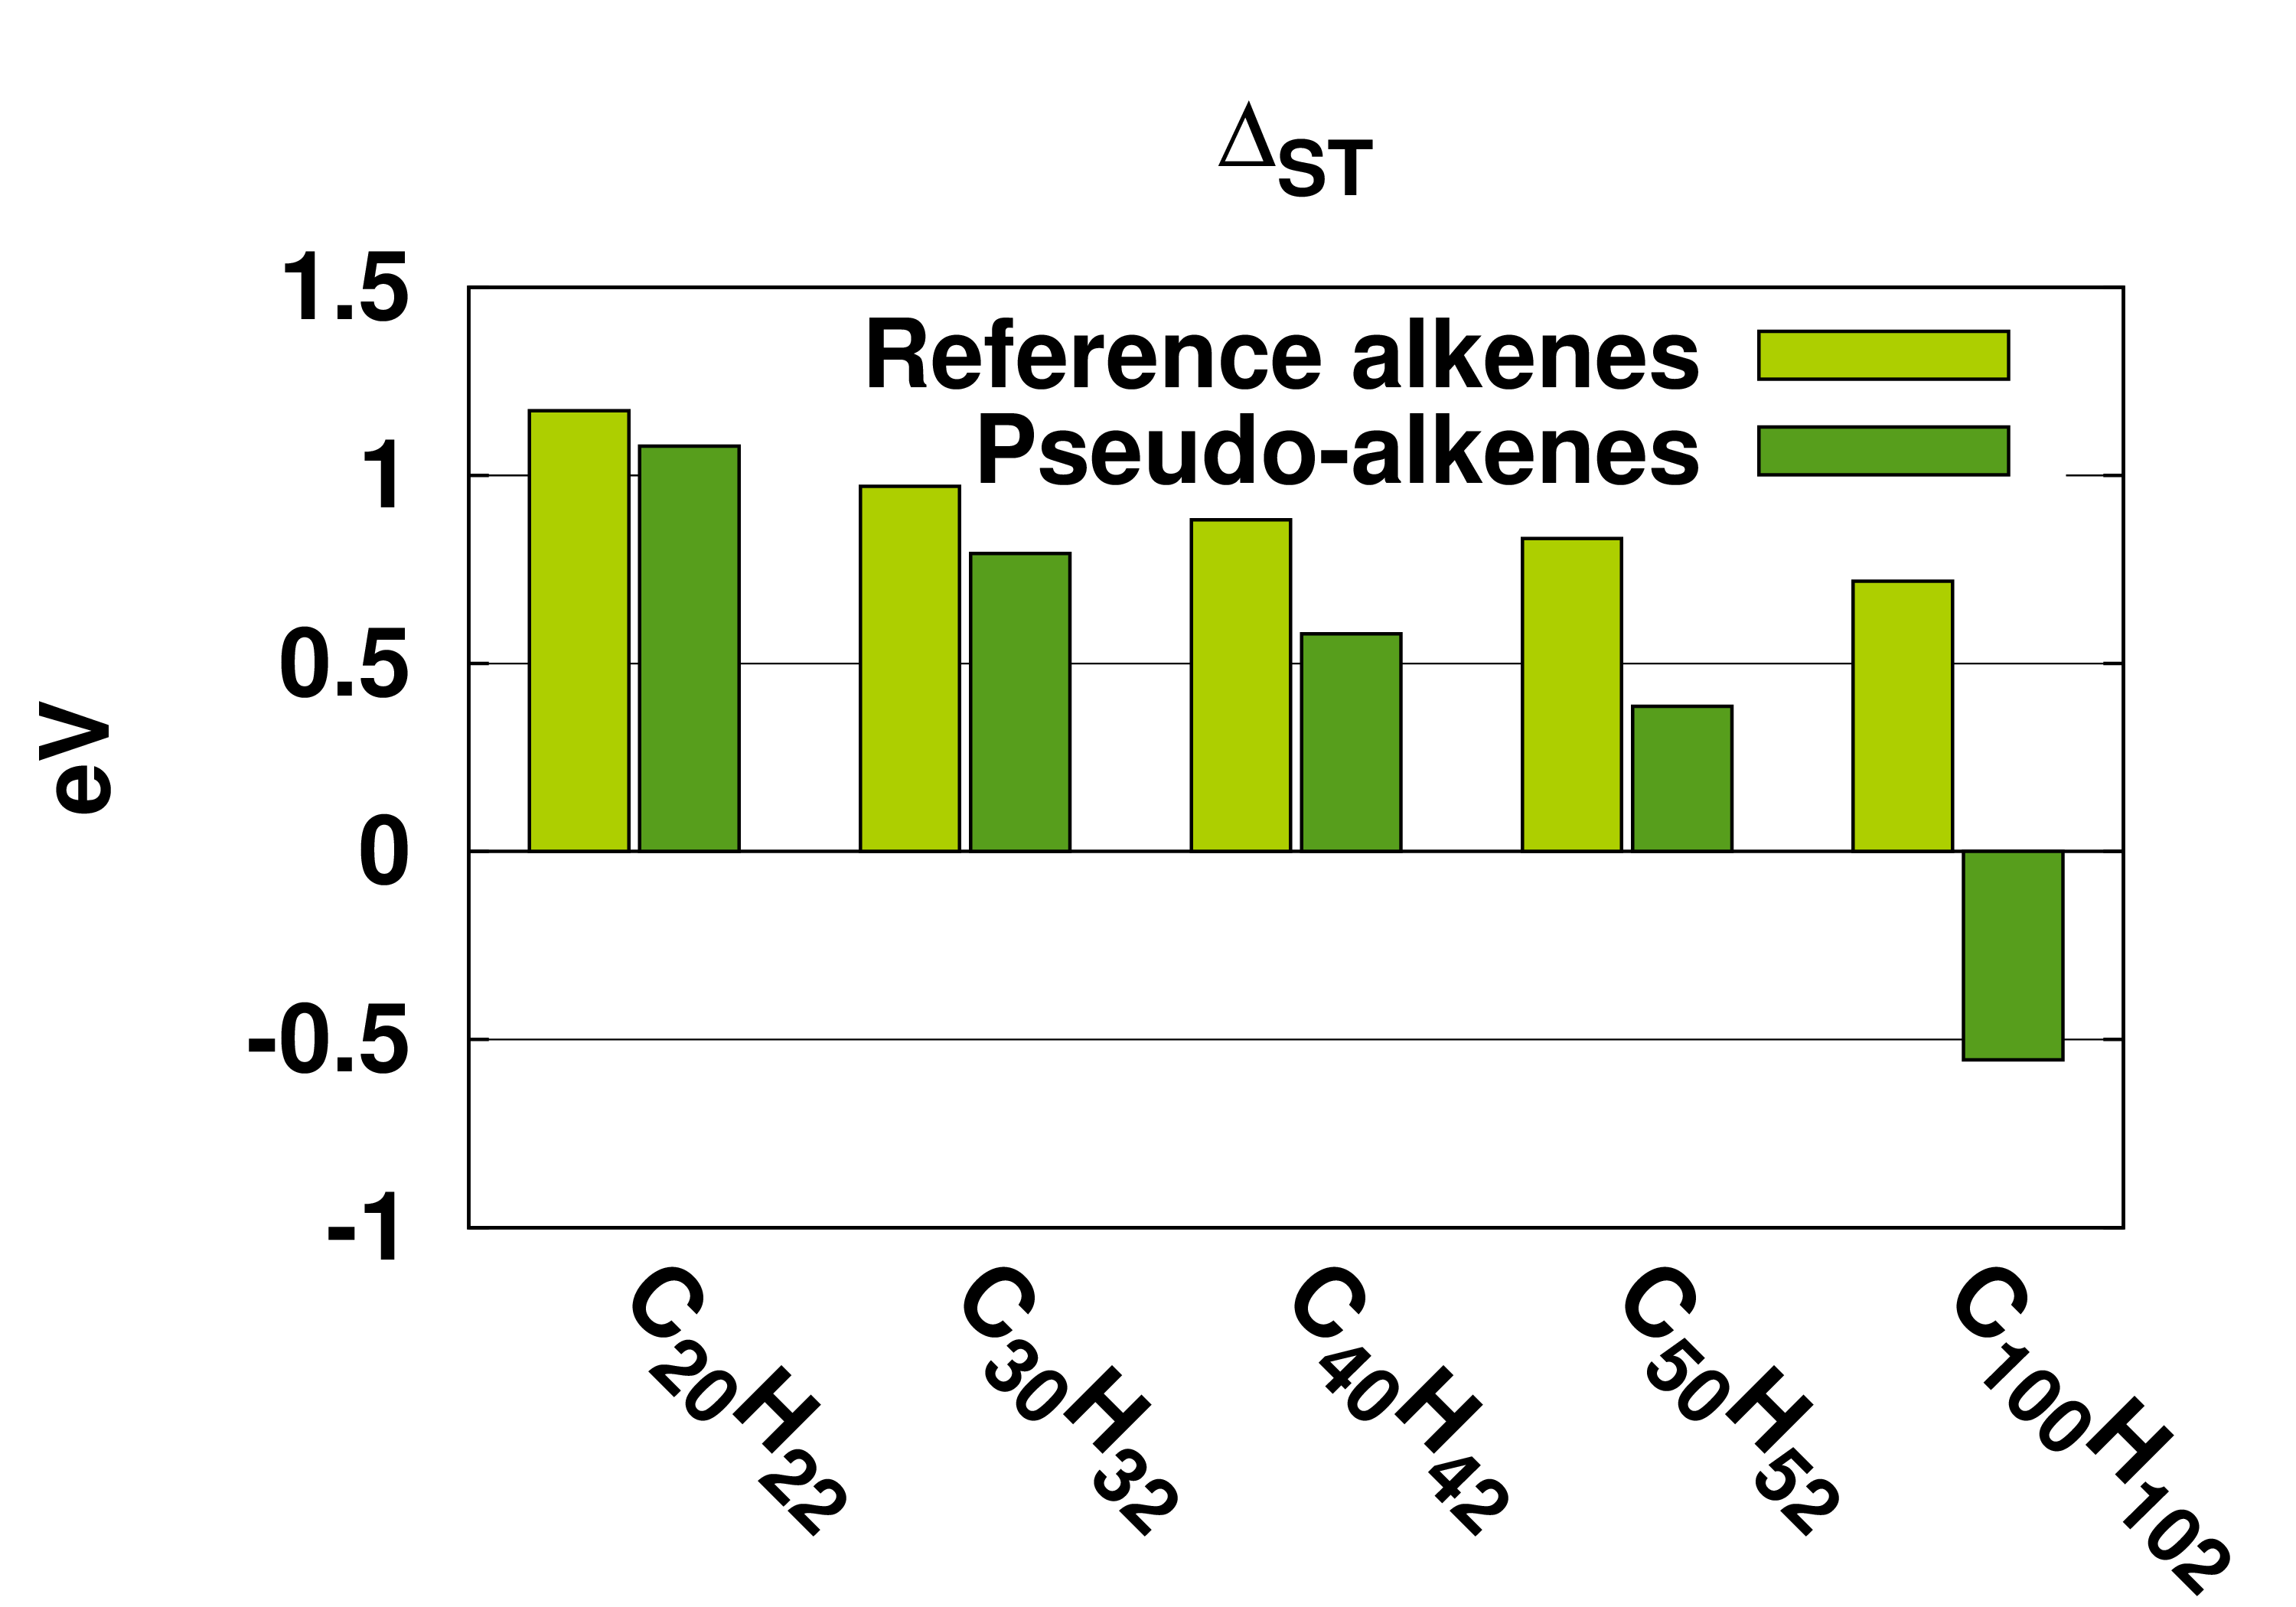
\includegraphics[width=7cm]{long_pbe0_st}
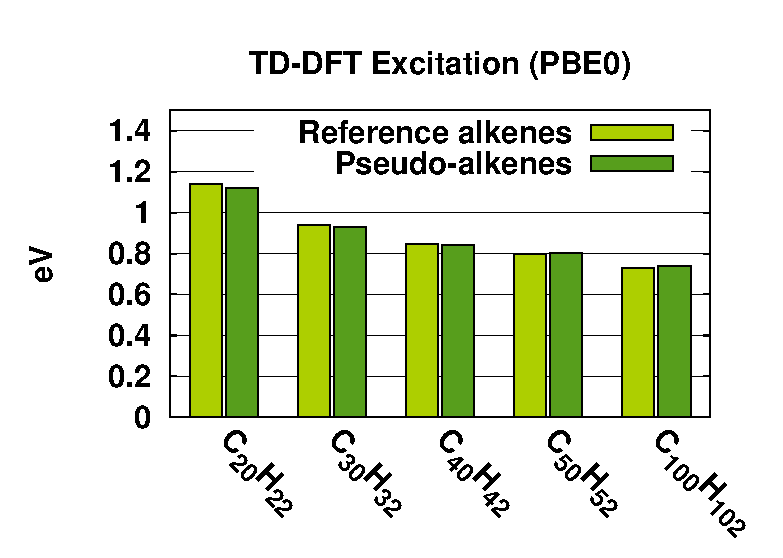
\includegraphics[width=7cm]{long_pbe0_tddft}
\end{center}

\caption{Comparison of the HOMO ($\varepsilon_{HOMO}$),
the ionisation (I.E.),
the first singlet-triplet $\pi-\pi^*$ excitation ($\Delta_{ST}$ and TD-DFT) energies
between the
all electron reference system and the optimal pseudo-potential across a range of long chain alkenes (C\(_{20}\)-C\(_{100}\)).
The $\Delta_{ST}$ values are the difference
between the lowest $\pi^*$  triplet (unrestricted formalism) and the lowest singlet state
(restricted formalism).
Calculations are at the PBE0/def-SV(P) level.}
\label{fig:long_chain_graphs}
\end{figure}

\begin{table}[ht]
\caption{Mean relative errors (in percent) across methods (HF or different functionals)
for long chain alkenes (C\(_{20}\)-C\(_{100}\)).
The basis set is def-SV(P).}
\begin{tabular}{l r r r r r }
\hline\hline
\%-error          & HF & PBE0 & PBE & TPSS & TPSSh \\
\hline
$\varepsilon_{HOMO}$    &  1.8 &  7.3   &  11.3   &  16.7    &  13.6 \\
I.E.                    & 25.1 &  6.7   &   9.4   &  10.3    &  11.6 \\
$\Delta_{ST}$           & 55.3 & 85.8   &  83.4   & 239.8    & 320.2 \\
TD-DFT $\pi-\pi^*$       & 30.1 &  1.0   &   6.1   &   5.6    &   2.9 \\ 
\hline\hline
\end{tabular}
\label{table:long_alkene_errors}
\end{table}

Figure~\ref{fig:long_chain_graphs} and Table \ref{table:long_alkene_errors} refer to longer 
alkene chains (\(n\) up to 100).
The pattern of decreasing ionisation energies and $\Delta_{ST}$ with increasing HOMO
energy is still followed, with the absolute error remaining consistent.
However, differences in the triplet-singlet energies between the reference and pseudo-systems 
become significant, notably for the largest case.
Here again, ionisation energy and $\epsilon_{HOMO}$ agree with mean average errors lower than
$10\%$ for PBE0.

Unlike for the previous systems, the larger the system, the larger the discrepancy between $\Delta_{ST}$
and TD-DFT results.
This apparent failure of the pseudo-potentials is to be found in the representation
of the triplet state.
The expectation values of the $S^2$ operator for the triplet calculations
are plotted in Figure \ref{fig:ssquare}, which shows that the spin contamination
of the triplet state computed as a single configuration (\emph{i.e.} in a SCF
framework) increases in both reference and pseudo-potential cases.
Yet, this effect is strengthened in the pseudo-potential calculations.
The triplet instability of the system represented with pseudo-potentials
is exacerbated.
As already shown, this is fixed by using the Tamm-Dancoff approximation,
as can be seen from the excellent agreement obtained with TD-DFT.\cite{tammdancoff}

\begin{figure}
\begin{center}
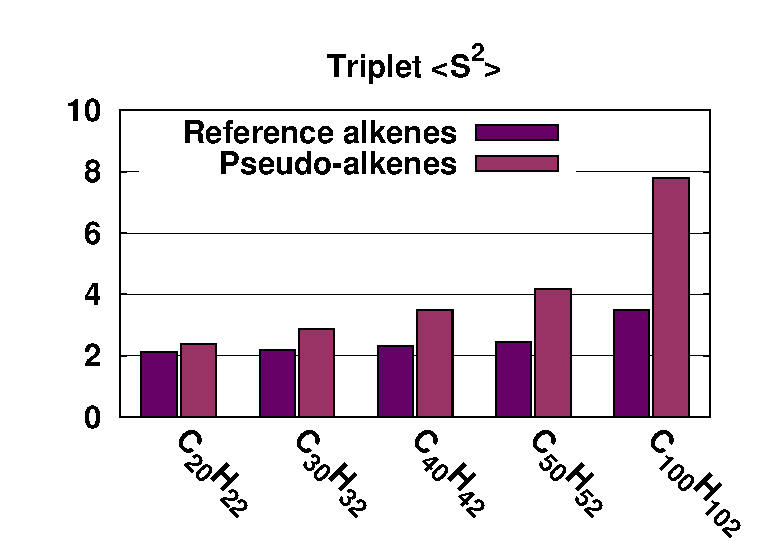
\includegraphics[width=8cm]{long_pbe0_s2}
\end{center}
\caption{Comparison of $S^2$ expectation values obtained for the calculation
of the first $\pi^*$ triplet configuration in a SCF formalism, for reference
and pseudo-systems.}
\label{fig:ssquare}
\end{figure}

\begin{table}[ht]
\caption{\label{tab:coef}Comparison of the weights (all electron \emph{vs.} pseudo-potentials)
of the excitations obtained with TD-DFT
to represent the triplet excited state from the closed shell singlet state.
Example case of C$_{50}$H$_{52}$.}
\begin{tabular}{c c r r}
\hline\hline
\multicolumn{2}{c}{Excitation} & \multicolumn{2}{c}{Weight(\%)}\\
\multicolumn{2}{c}{MO} & Ref. & Pseudo.\\
\hline
\multicolumn{2}{c}{25 a" \(\rightarrow\) 26 a"} & 77.0 &   67.1  \\
\multicolumn{2}{c}{24 a" \(\rightarrow\) 27 a"} & 10.5 &   13.1  \\
\multicolumn{2}{c}{23 a" \(\rightarrow\) 28 a"} & 3.6  &    5.2  \\
\hline\hline
\end{tabular}
\end{table}

In order to show that the recovering of the agreement between the pseudo-potential
and the reference calculations is not an artefact, we give in Table~\ref{tab:coef}
the weight and nature of each excitation (weight larger than 3\%)
in the description of the triplet excited state for
C$_{50}$H$_{52}$ (other values can be found in the SI, which exhibit the same trends).
As can be seen, the agreement is very good. 

These results show that the pseudo-potentials that we have extracted are able to reproduce the
$\pi$ systems in a variety of situations which are not part of their extraction set.
The molecular orbital virtual space is also well described (cf. Table~\ref{tab:coef}),
which demonstrates that the good agreement with reference calculations is
physically grounded.

\section{Conclusion}
In this work, we tackled the two main problems of the initial version of our
molecular potentials.
Firstly, the new pseudo-potentials for sp$^2$ hybridised
atoms are completely atomic and, even if the directionality of the bonding pattern
has to be fulfilled by correctly positioning the \(s\) potentials. No potentials need to
be added relative to the position of more than one atom.
Secondly, we gave a physical meaning to all the pseudo-potential
terms.
Contrary to our previous attempt, we do not rely on the "no collapse" term.
In fact, in this work we did not need such a term.
We could show that not only the occupied orbitals were well-reproduced
by the use of these new potentials, but also that the virtual space is of good quality
for excited states calculation.
The model defined here can be used in any quantum chemistry package which
implements atomic pseudo-potentials as we provide all the necessary parameters.
We are now working on extending our extraction method to other hybridised atoms
in order to provide a library of such potentials.

\section{Acknowledgments}
The authors acknowledge the french Minist\`ere de l'\'education
nationale et de la recherche for providing the PhD grant of A. Punter. The authors thank Prof St\'ephane Humbel and Dr Denis Hagebaum-Reignier for fruitful discussion.

\section{Supplementary materials}
In the supplementary materials are provided:
\begin{itemize}
\item a file containing discussions of the optimisation process used to generate the potentials, as well as of the computational gains found using the potential systems.
\item a spreadsheet file with all the calculated energies.
\item all the geometries used for the calculations.
\end{itemize}
%%%%%%%%%%%%%%%%%%%%%%%%%%%%%%%%%%%%%%%%%%%%%%%%%%%%%%%%%%%%%%%%%%%%%%%%%%%%%%%%%
% BIBLIOGRAPHY

\bibliography{biblio_pseudo_alex}   % Produces the bibliography via BibTeX.

\end{document}

